
\chapter{Metody kompensacji dyspersji}
\label{cha:comp_disp}
 
Istnieje wiele różnych metod kompensacji dyspersji w tej pracy szczegółowo opisane zostały wybrane trzy. Pierwsza polegająca na przygotowaniu sygnału, który sam skompensuje się do odpowiedniej postaci w trakcie propagacji. Druga bazująca na przybliżaniu krzywych dyspersji przy pomocy rozwinięcia w szereg Taylora, oraz trzecia polegająca na mapowaniu sygnału z dziedziny czasu na odległość 
 

\section{Cel kompensacji}
\label{sec:cel_komp}

\subsection{Zastosowanie fal Lamba w nieniszczacych testach}

Fale prowadzone akustyczne i ultradźwiękowe, w tym między innymi fale Lamba, są wykorzystywane na wiele sposobów między innymi do nieniszczących testów oraz oceny jakości obiektów. Stosowane są między innymi do diagnostyki uszkodzeń aktywnych lub pasywnych w monitorowaniu kondycji strukturalnej (SHM - Structural Health Monitoring). W niektórych przypakach fale te są wykorzystywane do uzyskania lokalnych informacji o próbce, której to informacji nie można uzyskać konwencjonalnymi technikami ultradźwiękowymi. Przykładem takiego zastosowania może być inspekcja spoiwa klejowego[2-Wilcox]. Jest to przykład aplikacji o krótkim zasięgu, ponieważ odległość propagacji fal kierowanych jest stosunkowo mała. Drugi obszar zastosowania kontroli fal prowadzonych jest przeznaczony do testowania dalekiego zasięgu. W tym przypadku odległość propagacji jest stosunkowo duża. Ich główną zaletą, sprawiającą, iż są one tak często wykorzystywane do diagnozy urządzeń jest to, że mogą być wzbudzane przez elementy uruchamiające znajdujące się na lub wewnątrz struktury w jednym punkcie konstrukcji i mogą się rozprzestrzeniać na duże odległości. Konwencjonalna kontrola ultradźwiękowa dużych struktur jest bardzo czasochłonna, ponieważ testom musi zostać poddany każdy punkt badanej struktury, która ma być monitorowana. Wykorzystanie fal Lamba jest więc potencjalnie bardzo atrakcyjnym rozwiązaniem tego problemu. Jeżeli przetwornik odbierający znajduje się w odległym punkcie struktury, odebrany sygnał zawiera informacje o całej przebytej ścieżce propagacji między przetwornikami nadawczym i odbiorczym. W związku z tym test monitoruje całą ściężkę, a nie pojedynczy punkt struktury. Pozwala to na znaczne zaoszczędzenie czasu badań. W przypadku prętów niejednokrotnie stosuje się techniki, w których nadajnik po wyemitowniu sygnału przełącza się w tryb odbiornika. Propagujący sygnał odbija się od końca pręta i wraca spowrotem, gdzie jest odbierany i może zostać poddany analizie. Takie podejście jest bardzo często stosowane, zwłaszcza w sytuacjach, w których dostęp do pręta możliwy jest tylko z jednej strony jak na przykład podczas badania kotw górniczych. Przykład ich położenia ilustruje rysunek \ref{fig:kotwy}
\begin{figure}[h]
\centering
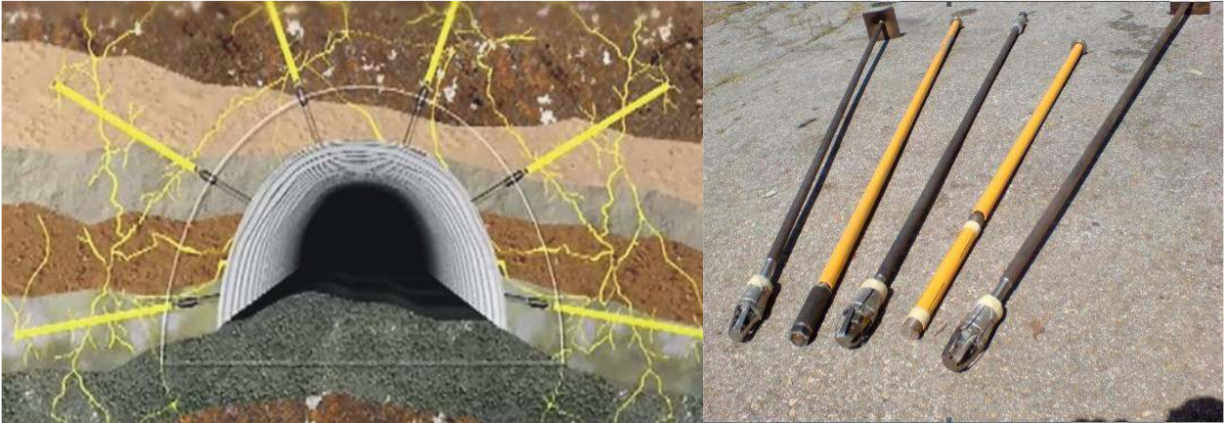
\includegraphics[width=14cm]{Zdjecia/4/kotwy}
\caption{Przykład zamontowania kotw górniczych, do których dostęp w przypadku testów jest tylko z jednej strony \ref{art:kotwy}}
\label{fig:kotwy}
\end{figure}

Nawet w najprostszych strukturach, takich jak swobodna płaska izotropowa płyta lub prosty stalowy pręt, może istnieć nieskończona liczba sterowanych trybów falowych. Co więcej, postaci te są generalnie dyspersyjne. Obydwa te fakty utrudniają praktyczne zastosowanie fal kierowanych. W praktyce testy kontroli dalekiego zasięgu są wykonywane w sposób zadowalający, gdy stosuje się tylko jedną lub czasami dwie postaci fal prowadzonych, a pozostałe są tłumione. Tradycyjnie osiąga się to za pomocą specjalnych przetworników. Dzięki starannej kontroli częstotliwości i liczby falowej wzbudzenia, możliwe jest generowanie wybranych postaci fali Lamba oraz tłumienie pozostałych. Kontrola zakresu częstotliwości może być osiągnięta przez użycie sygnału o pewnej szerokości pasma zamkniętego w oknie Hanninga lub Gaussa. Zakres liczby falowej może być ograniczony przez użycie starannie zaprojektowanych sond EMAT lub za pomocą piezoelektrycznego przetwornika. 

Powyższe metody mogą służyć do tłumienia sygnałów wywołanych przez niepożądane postaci fali, ale nie mogą zapobiec efektowi dyspersji, ponieważ zjawisko to występuje w falach kierowanych podczas ich propagacji w strukturze. Dyspersja sygnału powoduje, rozproszenie energii sygnału w czasie i przestrzeni w trakcie propagacji sygnału. W praktyce objawia się to wzrostem czasu trwania odbieranego sygnału w porównaniu do czasu trwania sygnału wejściowego. Rysunek \ref{fig:dyspersja} ilustruje przykład sygnału bez dyspersji oraz sygnału rozproszonego na skutek propagacji pewnej odległości. Łatwo zauważyć, że sygnał przed propagacją trwa zaledwie $0,0001 s$ natomiast po jego czas zwiększa się do około $0,0013s$ a zatem trwa ponad 10 razy dłużej.
\begin{figure}[h]
\centering
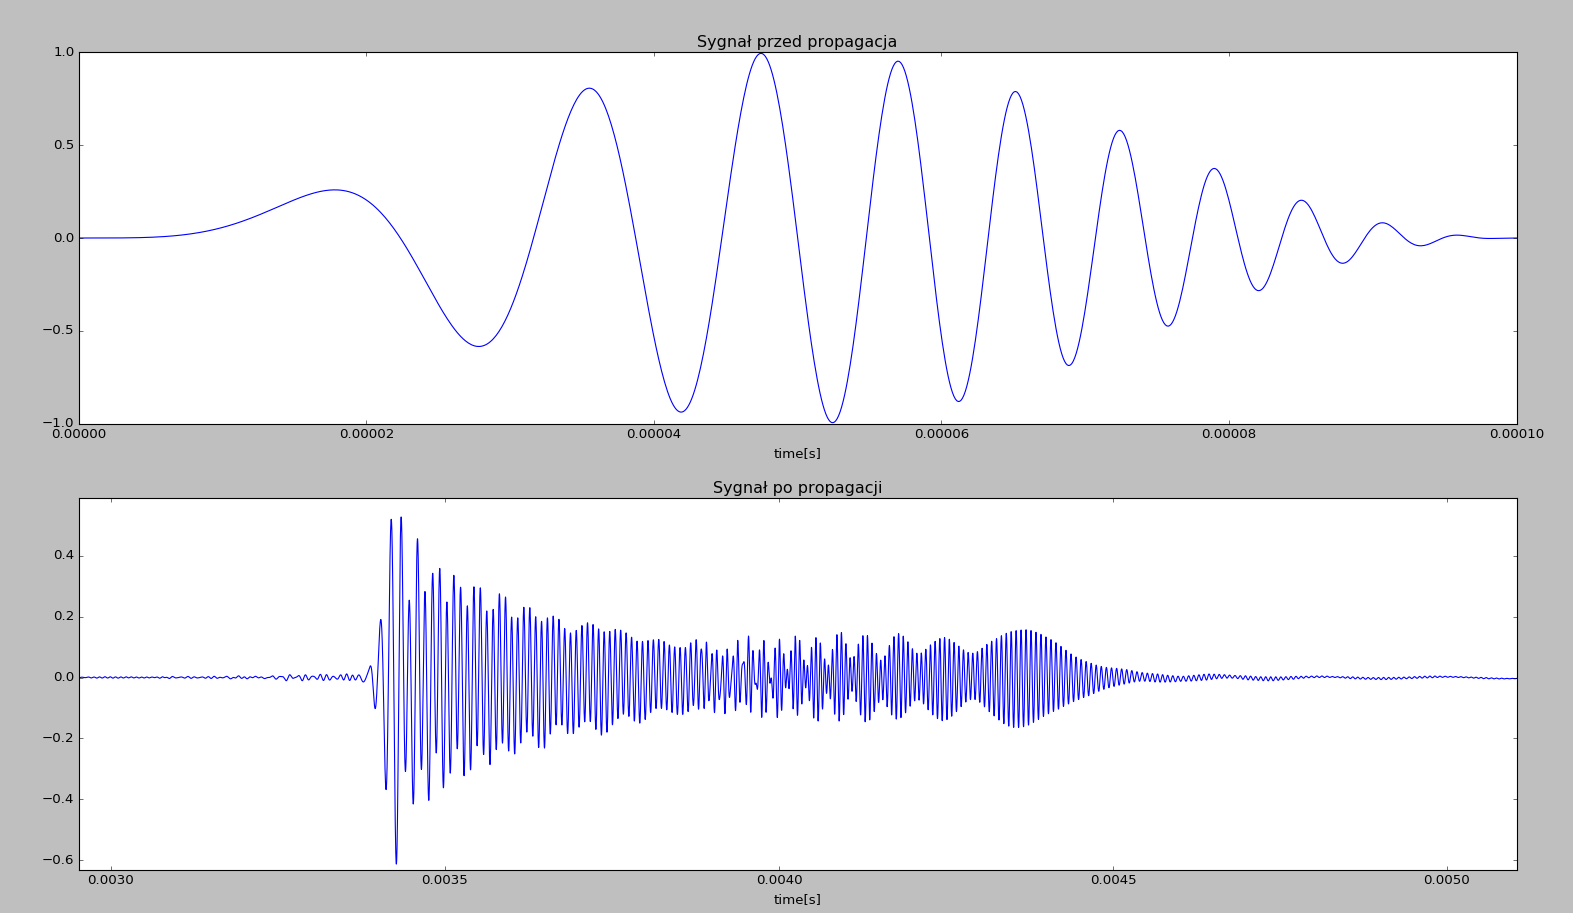
\includegraphics[width=14cm]{Zdjecia/4/dyspersja}
\caption{Przykład sygnału wejściowego, oraz sygnału rozproszonego}
\label{fig:dyspersja}
\end{figure}

 Zjawisko to pogarsza rozdzielczość i sprawia, że dane eksperymentalne są trudne do interpretacji z powodu nakładania się sygnałów. Używanie sygnałów wejściowych o określonej przepustowości może zmniejszyć problem dyspersji. Takie podejście koncentruje energię wejściową w ograniczonym zakresie częstotliwości, w którym jakiekolwiek zmiany prędkości pożądanego trybu fal kierowanych są małe. W praktyce oznacza to pracę w punktach na krzywych dyspersji dla konkretnego układu, w których prędkość grupowa jest stacjonarna lub prawie stacjonarna względem częstotliwości. Takie punkty zostały określone jako punkty "zerowej dyspersji" w\textcolor{red}{[1kasia]}, jest to określenie, które może wprowadzać w błąd, ponieważ niemożliwe jest skoncentrowanie całej energii sygnału wejściowego o skończonej długości na jednej częstotliwości. Zostało udowodnione \textcolor{red}{[2kasia]}, że istnieje optymalny sygnał wejściowy dla każdego punktu na krzywych dyspersji, który maksymalizuje rozdzielczość, jaką można uzyskać w tym punkcie. Jeśli jednak przyjmiemy, że przetwarzanie sygnału jest dozwolone przed wyświetlaniem informacji operatorowi, możliwe jest inne podejście do fal prowadzonych oraz ich roli w nieniszczących testach.

Należy również zaznaczyć, iż w praktyce rozproszone sygnały są zwykle uszkodzone z powodu szumów. Zachodzące na siebie i słabnące sygnały w porównaniu z szumem sprawiają, że dane z czujników są trudniejsze do interpretacji. W konsekwencji rodzielczość może ulec pogorszeniu. Dlatego zrodziła się ogromna potrzeba opracowania technik przetwarzania sygnałów w celu zwiększenia rozdzielczości czasowej i amplitudy SNR.

Z punktu widzenia systemów SHM, kompresja sygnału lub usuwanie dyspersji w dziedzinie czasu może być wygodnym i intuicyjnym sposobem na łatwiejszą interpretację sygnałów czujnika.

\subsection{Sygnał stosowany wy symulacji}
W ramach niniejszej pracy powstała aplikacja, pozwalająca użytkownikowi na podstawie podanych parametrów pręta wygenerować krzywe dyspersji opisujące dany obiekt. Aplikacja pozwala również na wygenerowanie sygnału testowego, symulację jego propagacji w zadanym pręcie, oraz kompensację otrzymanego sygnału wybranymi metodami. Sygnałem stosowanym do testów był sygnał chirp zmodyfikowany przypomocy okna Hanninga.
	Sygnał o nazwie chirp jest sygnałem sinusoidalnym, w którym faza jest funkcją czasu. \textcolor{red}{[3kasia]}. Sygnał o nazwie linear chirp to sygnał, w którym częstotliwość zmienia się w sposób liniowo zależny od czasu. Sygnał taki jest opisany wzorem:
	\begin{equation}
	s(t) = \sin(\phi (t))
	\end{equation}
	
	Gdzie $\phi (t)$ to funkcja fazy. Chwilową częstotliwość takiego sygnału jest związana funkcją fazy następującą zależnością:
	\begin{equation}
	f(t) = \frac{1}{2\pi}\frac{d(\phi (t))}{dt} \label{eq:f(t)_z_phi}
	\end{equation}
	
	Aby zatem wygenerować sygnał linear chirp o rządanych parametrach należy przyjąć, iż funkcja częstotliwości przybiera postać:
	\begin{equation}
	f(t) = f_0+\frac{B}{T}t \label{eq:f(t)_liniowo}
	\end{equation}
	
	Gdzie:
	
	$f_0$ - częstotliwość początkowa
	
	$B$ - szerokość pasma częstotliwości
	
	$T$ - czas trwania sygnału
	
	Łącząc równania (\ref{eq:f(t)_z_phi}) oraz (\ref{eq:f(t)_liniowo}) można funkcję fazy zapisać jako:
	\begin{equation}
	\phi (t) = 2\pi f_0t+\frac{\pi Bt^2}{T} \label{eq:phi(t)}
	\end{equation}
	A zatem pełen wzór opisujący sygnał linear chirp można zapisać jako:
	\begin{equation}
	s(t) = \sin(2\pi f_0t+\frac{\pi Bt^2}{T})
	\end{equation}
	
	Przykład funkcji częstotliwości oraz uzyskanego w ten sposób sygnału przedstawia rysunek \ref{fig:linear_chirp}
\begin{figure}[h]
\centering
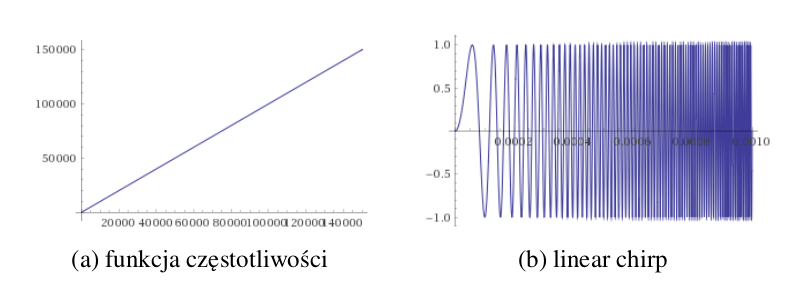
\includegraphics[width=14cm]{Zdjecia/4/linear_chirp}
\caption{Przykład sygnału linear chirp (b) oraz jego funkcji częstotliwości (a)}
\label{fig:linear_chirp}
\end{figure}

W prezentowanej pracy, sygnałem, który był poddawany symulacji był liniowy chirp dodatkowo pomnożony przez funkcję okna Hanninga daną wzorem:
\begin{equation}
w(n)=0,5(1-cos(\frac{2\pi n}{N-1})) \label{eq:okno_hanninga}
\end{equation}

Gdzie $N$ to całkowita liczba próbek. uzyskany w ten sposób sygnał został zaprezentowany na rysunku \ref{fig:test_chirp}
\begin{figure}[h]
\centering
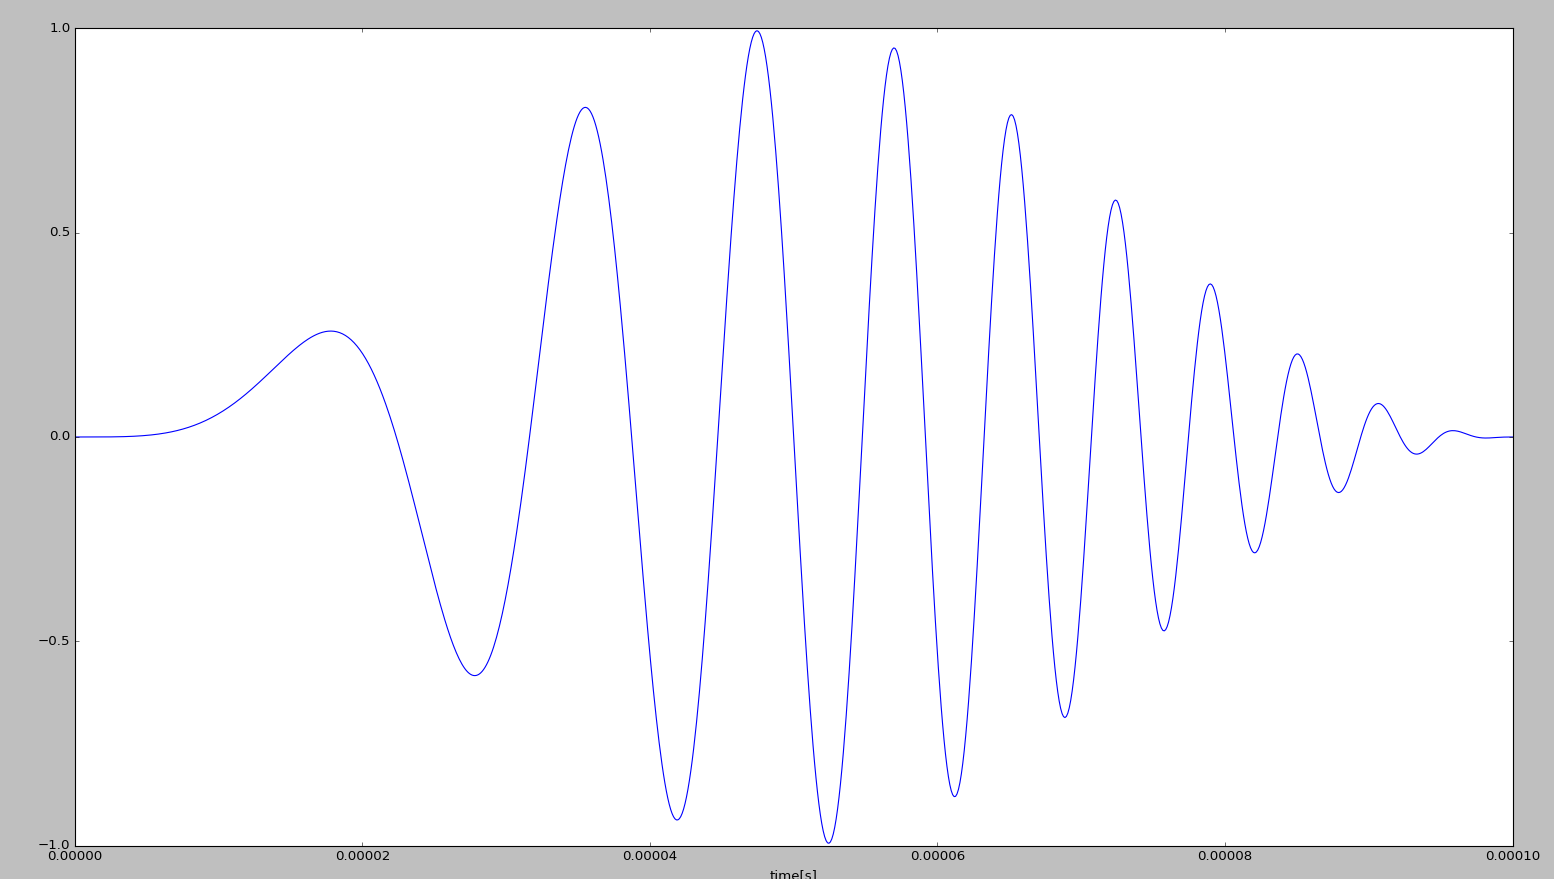
\includegraphics[width=14cm]{Zdjecia/4/test_chirp}
\caption{Linear chirp pomnożony przez funkcję okna Hanninga}
\label{fig:test_chirp}
\end{figure}

W aplikacji zaimplementowany został algorytm generujący opisany wyżej sygnał o następujących parametrach:

\begin{itemize}
\item czas trwania sygnału - 0.0001s
\item częstotliwość minimalna - 0Hz
\item częstotliwość maksymalna - 100kHz
\end{itemize}

Całość stworzona jest w oparciu o koncepcję otwartego koduco daje użytkownikowi możliwość pisania własnych funkcji, generujących dowolne sygnały a następnie ich bezproblemową symulcję w stworzonej aplikacji.

\section{Agregacja krzywych dyspersji uzyskanych z zaimplementowanego solvera}
\label{sec:agregacja}

\subsection{Cel agregacji}
Podstawą opracowania każdej z przedstawionych w tej pracy metod kompensacji jest znajomość krzywych dyspersji badanego obiektu, jakim jest stalowy pręt. Stanowią one pewnego rodzaju funkcję przejścia sygnału pomiędzy jednym punktem w czasie i przestrzeni a dowolnym innym punktem. Ich znajomość stanowi więc klucz do skompensowania efektu dyspersji. W stworzonej aplikacji, dzięki zastosowaniu odpowiednich algorytmów oraz na podstawie odpowiednich zadanych parametrów badanego obiektu, otrzymywane są poszukiwane krzywe dyspersji. Jednak dane są one w postaci chmury punktów zapisywanych w odpowiednich plikach. Aby funkcje te nadawały się do użycia należy każdy z wygenerowanych punktów przypisać do odpowiadającej krzywej. W ten sposób uzyskane zostaną funkcje, z których każda opisywać będzie zachowanie innej postaci fali prowadzonej. Przykładowe wygenerowane krzywe dyspersji przed agregacją przedstawia rysunek 2.21

\subsection{Algorytm agregacji}
 Krzywe dyspersji wyrażają zależność liczby falowej od częstości kątowej. Jako wynik w aplikacji otrzymujemy pojedynczy wektor zawierający kolejne wartości liczby falowej oraz zestaw odpowiadających danej liczbie częstości kątowych. Pierwszym krokiem w agregacji tak zapisanych danych jest zapisanie wszystkich danych w postaci chmury punktów o dwóch współrzędnych $A=(\omega , k)$ oraz posortowanie ich rosnąco wartościami $\omega$. Liczba wygenerowanych krzywych odpowiada ilości punktów posiadających tę samą współrzędną k. Ponieważ są to wartości własne równania (2.44) to dla każdej wartości k jest ich tyle samo. Każda krzywa składa się z dokładnie takiej liczby punktów jaka jest długość wektora k. Kolejnym krokiem jest przyporządkwanie pierwszych dwóch punktów do każdej z krzywych. Mając punkty uporządkowane względem $\omega$ wystarczy wybrać te o najmniejszej wartości k. Każdy z nich odpowiada kolejnemu trybowi fali. Punkty przydzielone do właściwego trybu zostają usunięte ze zbioru punktów do przydzielenia. Analogicznie postępujemy w przypadku drugiej grupy punktów. Wybieramy te o najniższej wartości k i przypisujemy do poszczególnych trybów. Agregacja kolejnych punktów musi przebiegać według innego schematu, ponieważ krzywe się wzajemnie przecinają i segregacja względem częstotliwości nie przyniesie zadowalających rezultatów. Przyjmując, że dla dowolnego modu, ostatni zagregowany punkt ma współrzędne $P_l = (\omega _l,k_l)$ z chmury punktów wybieramy zbiór potencjalnych punktów spełniających następujące warunki:
 \begin{enumerate}
 \item Wartość k potencjalnych punktów musi wynosić $k=k_p=v_k[l+1]$
 
 Gdzie $k_p$ oznacza wartość k potencjalnych punktów, $v_k$ oznacza posortowany rosnąco wektor wartości k, a $l+1$ to indeks wartości z wektora $v_k$ o jeden większy niż indeks ostatnio zagregowanego do danego trybu punktu
 \item Wartość $\omega$ potencjalnych punktów musi znajdować się w pewnym, ograniczonym otoczeniu wartości $\omega _l$
 
 Ze zbioru potencjalnych punktów, które spełniają wyżej wymienione warunki należy następnie wybrać ten, który w najepszy sposób będzie pasował do powstałego już fragmentu krzywej dyspersji. W celu wybrania najlepszego punktu obliczony zostaje kąt pomiędzy wektorami $\overrightarrow{v_1} = \overrightarrow{P_{l-1}P_l}$ oraz $\overrightarrow{v_2} = \overrightarrow{P_lP_{p_i}}$, gdzie $P_{p_i}$ oznacza i-ty potencjalny punkt ze zbioru. Sformułowanie najlepiej pasujący punkt oznacza, iż kąt pomiędzy rozważanymi wektorami, obliczany ze wzoru:
 \begin{equation}
 \alpha = \arccos\frac{\overrightarrow{v_1} \circ \overrightarrow{v_2}}{|\overrightarrow{v_1}|\cdot|\overrightarrow{v_2}|}
\end{equation}  
ma wartość najbliższą zeru. Usuwając zagregowane już punkty ze zbioru punktów do przydzielenia oraz postępując w sposób analogiczny do przedstawionego schematu, wszystkie punkty ze zbioru zostają przydzielone odpowiedniej krzywej. Wyniki agregacji zostały przedstawione na rysunku \ref{fig:krzywe_po_agregacji}
 
\begin{figure}[h]
\centering
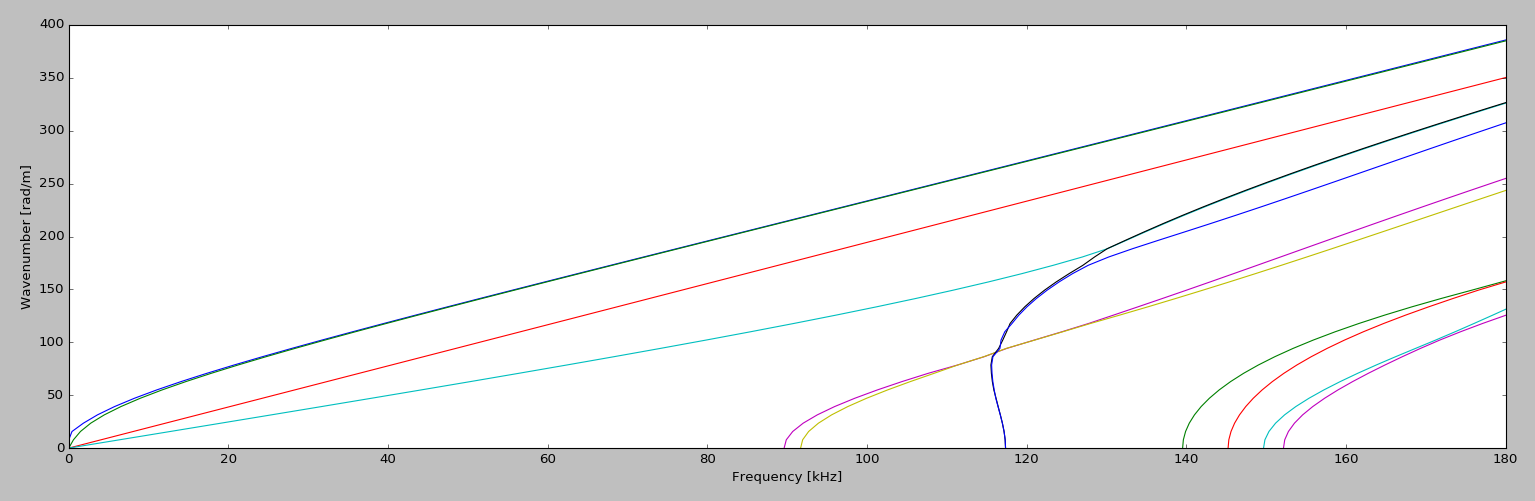
\includegraphics[width=13cm]{Zdjecia/4/zagregowane_krzywe}
\caption{Krzywe dyspersji po agregacji}
\label{fig:krzywe_po_agregacji}
\end{figure}
\end{enumerate}  

Jak łatwo zauważyć opisany algorytm w sposób efektywny agreguje chmurę punktów do odpowiednich krzywych. Uporządkowoane w ten sposób punkty zostały wykorzystane do opracowania trzech metod kompensacji, opisanych w kolejnych sekcjach tego rozdziału.





\section{Metoda odwracania sygnału w czasie}
\label{sec:metoda_tr}

Metoda omawiana w tej sekcji polega na wygenerowaniu sygnału który po przepropagowaniu pewnej odległości sam się skompensuje. Technika kompensacji dyspersji poprzez wygenerowanie sygnału odwróconego w czasie została zaprezentowana w artykule \cite{kasia4}

\subsection{Podstawy teoretyczne}
Podstawową ideą prezentowanej w tej części pracy techniki kompensacji dyspersji jest wytworzenie sygnału, który poprzez nałożenie składowych częstotliwości w czasie propagacji skompensuje się, tworząc oczekiwany sygnał w pozycji pomiarowej. W przypadku w którym do obiektu wprowadzony zostanie zwykły sygnał sinusoidalny o liniowo zmieniającej się częstotliwości (linear-chirp) zostanie wzbudzone przynajmniej kilka trybów fali prowadzonej. Każdy tryb w każdej z częstotliwości może poruszać się z różną prędkością fazową i grupową. Ze względu na dyspersję sygnał wraz z propagacją będzie stawał się coraz dłuższy a jego amplituda będzie spadać, ponieważ ulegnie on rozproszeniu.  Składowe częstotliwości sygnału odpowiadające najwyższym prędkością grupowym będą znajdować się z przodu, natomiast wolniejsze komponenty będą znajdowały się z tyłu. Podstawa przedstawianej metody polega na założeniu, że tak otrzymany sygnał jesteśmy w stanie odwrócić w czasie, tak aby komponenty o mniejszej prędkości znalazły się z przodu sygnału a komponenty o większej prędkości znalazły się z tyłu. Wzbudzenie obiektu tak przygotowanym sygnałem da w odpowiedzi sygnał skompensowany tej samej postaci co pierwotne wzbudzenie. Skuteczność metody można wykazać analitycznie. Przyjijmy, że sygnał zastosowany do wzbudzenia pręta zostanie zastosowany w punkcie $x = 0$ i będzie to sygnał $f(t)$. Sygnał wzbudzający w dziedzinie częstotliwości możemy zapisać jako:
\begin{equation}
[F(\omega)_{x=0}]=\int\limits_{-\infty}^{\infty}f(t)e^{-i\omega t}dt \label{eq:F(omega)_x=0}
\end{equation}
Jeśli przez nasz obiekt propaguje jedna postać fali to w punkcie $x=L$ można tę funkcję zapisać jako:

\begin{equation}
[F(\omega)_{x=L}]=\int\limits_{-\infty}^{\infty}f(t)e^{-i(\omega t - kL}dt \label{eq:F(omega)_x=L}
\end{equation}

gdzie liczba falowa k jest funkcją częstotliwości $\omega$  , która jest opisana za pomocą krzywej dyspersji dla danego trybu fali. Równania (\ref{eq:F(omega)_x=0}) oraz (\ref{eq:F(omega)_x=L}) można powiązać funkcją przejścia $H(\omega)$ co można zapisać jako:
\begin{equation}
H(\omega) = \frac{[F(\omega)]_{x=L}}{[F(\omega)]_{x=0}} \label{eq:h(omega)}
\end{equation}

Zakładając, że chcemy uzyskać sygnał $g(t)$, którego transformata Fouriera to $G(\omega)$ przy ($x = L$) wtedy wymagany sygnał wejściowy ($x = 0$) $Y(\omega)$:
\begin{equation}
Y(\omega) = \frac{G(\omega)}{H(\omega)} = G(\omega)[H(\omega)]^{-1} \label{eq:Y(omega)}
\end{equation}
Sygnał w dziedzinie czasu y(t) jaki musi zostać wprowadzony do badanego pręta w punkcie $x=0$ aby uzyskać odebrany sygnał $g(t)$ w punkcie $x=L$ można uzyskać z odwrotnej transformaty Fouriera, co pokazuje równanie (\ref{eq:Y(omega)}):
\begin{equation}
y(t) = \frac{1}{2\pi}\int\limits_{-\infty}^{\infty}\frac{G(\omega)}{H(\omega)}e^{i\omega t}d\omega \label{eq:y(t)}
\end{equation}

W prostym przypadku gdy analizujemy pojedynczą postać fali prowadzonej:
\begin{equation}
[H(\omega)]^{-1} = e^{-ikL} = e^{-i\omega L/c}
\end{equation}
\begin{equation}
y(t) = \frac{1}{2\pi}\int\limits_{-\infty}^{\infty}G(\omega)e^{-i\omega (L/c - t)}d\omega
\end{equation}

Przyjmując, że sygnał w domenie czas $g(t)$ jest aplikowany w punkcie $x = 0$ sygnał $y^*(t)$ w punkcie x = L można zapisać jako:
\begin{equation}
y^*(t) = \frac{1}{2\pi}\int\limits_{-\infty}^{\infty}G(\omega)e^{-i\omega (L/c + t)}d\omega
\end{equation}

Technika kompensacji w tym przypadku polega na odebraniu sygnału $y^*(t)$ w przedziale czasowym $t\in [0,T]$ w którym cała paczka falowa zostanie odebrana przez odbiornik. Następnie sygnał zostaje odwrócony w czasie. Otrzymany w ten sposób sygnał może być zaaplikowany do badanego pręta. W trakcie propagacji zostanie on skompensowany do fali o kształcie takim jak kształt sygnału $g(t)$

\subsection{Implementacja numeryczna}
W ramach niniejszej pracy, omawiana metoda została zaimplementowana do aplikacji. Podstawa jej działania opiera się na znajomości krzywych dyspersji. Pierwszym etapem jest wygenerowanie sygnału, jaki chce się uzyskać w wyniku kompensacji. Następnie dzięki zaimplementowanym metodom należy uzyskać przewidywany kształt sygnału po przepropagowaniu zadanej odległości oraz odrócenie go w czasie. Sygnał otrzymany z tak przygotowanego sygnału wejściowego powinien skompensować się na zadanej odległości. Rysunek \ref{fig:kolejne_etapy_TR} przedstawia opisane kroki na przykładzie sygnału linear chirp.
\begin{figure}[h]
\centering
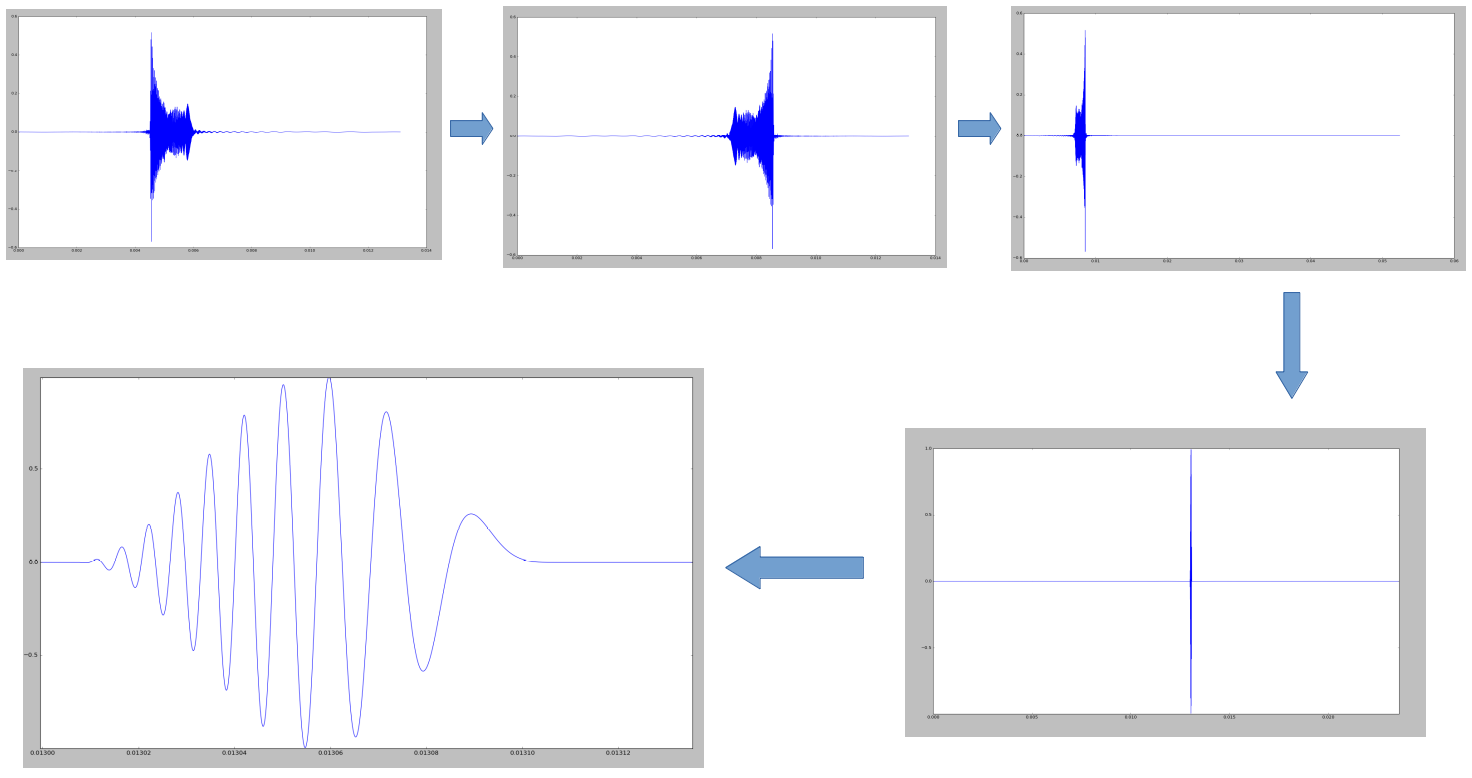
\includegraphics[width=14cm]{Zdjecia/4/algorytm_komp_tr}
\caption{Algorytm kompensacji odwracania czasu}
\label{fig:kolejne_etapy_TR}
\end{figure}

W zaprezentowanym przykładzie odwrócony w czasie sygnał został dodatkowo wypełniony zerami. Zabieg ten został zastosowany, ponieważ całość została przeprowadzona w ramach symulacji i wypełnienie sygnału było konieczne do przeprowadzenia prawidłowej symulacji propagacji. Przedstawiana metoda pozwala zatem wygenerować sygnał kompensujący się na zadanej odległości do fali o oczekiwanym kształcie. Pozwala na propagowanie zarówno pojedynczego trybu jaki nałożonych wielu postaci fali prowadzonej. Jednak aby móc stosować tę motodę konieczna jest znajomość długości ścieżki propagacji sygnału. Jeżeli ściażka propagacji ulegnie zmianie, konieczne jest wygenerowanie nowego sygnału adekwatnego do aktualnego badanego obiektu. W przypadku w którym podczas propagacji następowałyby dodatkowe odbicia, na przykład w sytuacji, w której fala propagujące przez dwa pręty złączone ze sobą, część energii zostanie odbita od punktu złączenia a część przepropaguje przez drugi pręt i odbije się na końcu. Stworzenie sygnału kompensującego się w takiej sytuacji byłoby bardziej skomplikowane i nie zostało opisane w tej pracy. Rysunek \ref{fig:rozne_odl} prezentuje przykład fali przygotowanej do kompensacji po 4 metrach propagacji, który przepropagował kolejno 1,2,4 i 5 metrów.

\begin{figure}[h]
\centering
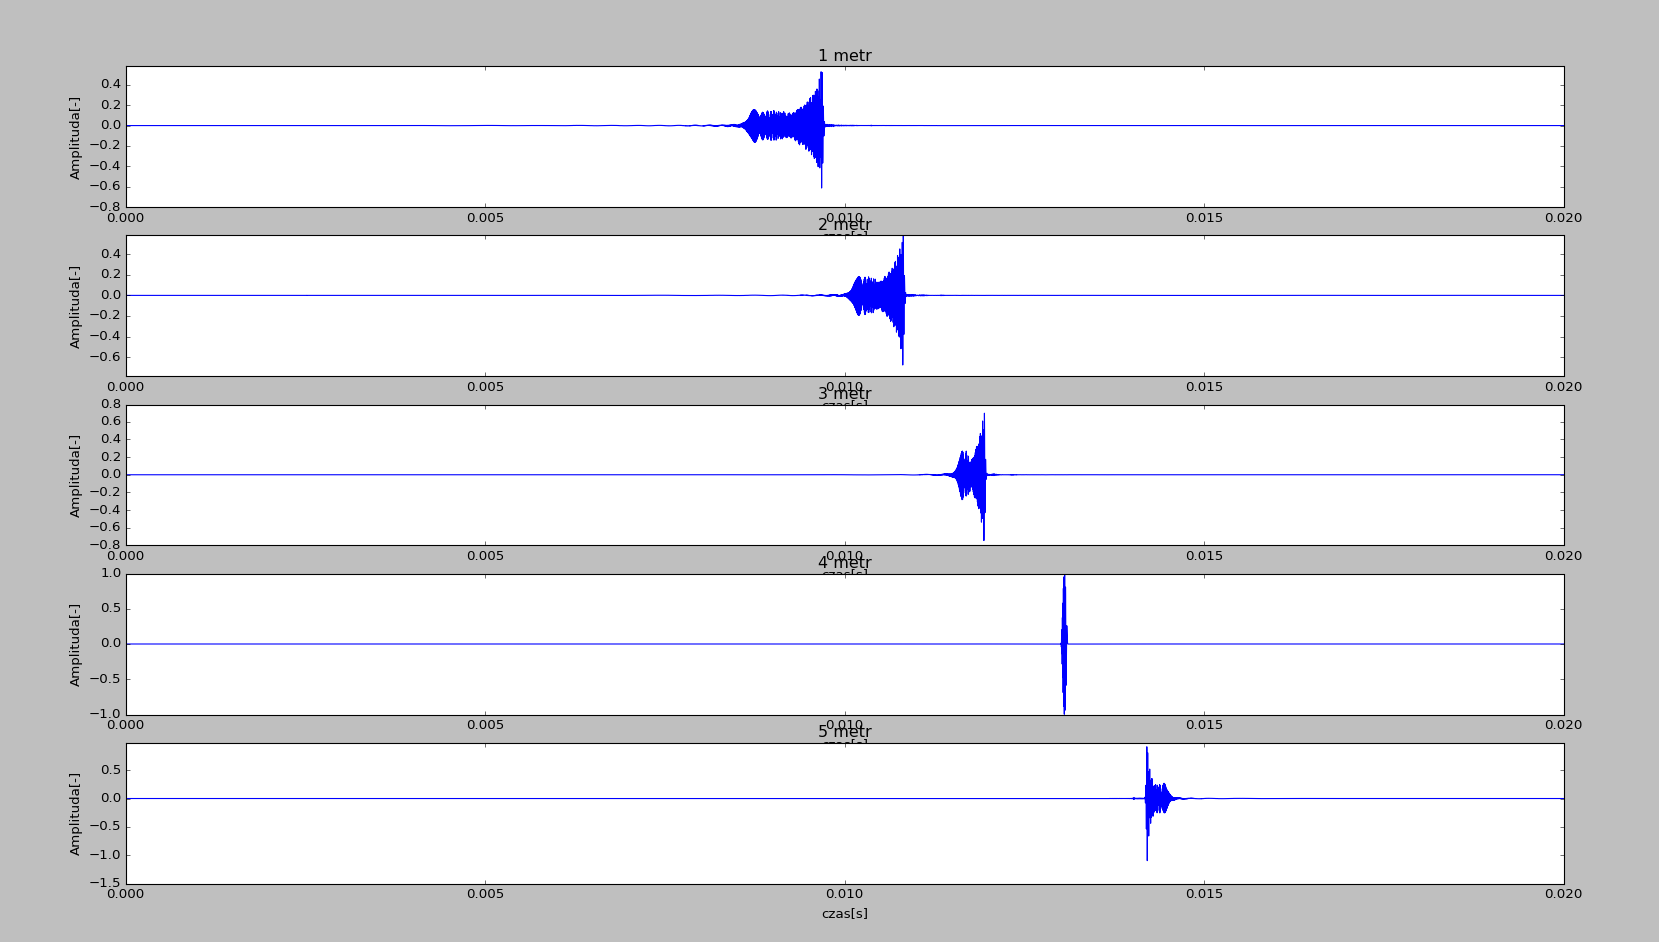
\includegraphics[width=14cm]{Zdjecia/4/porownanie_roznych_odleglosci_time_reversal}
\caption{Sygnał przygotowany do kompensacji po 4 metrach propagacji przedstawiony kolejno po 1, 2, 4 i 5 metrach propagacji}
\label{fig:rozne_odl}
\end{figure}

Jak łatwo zauważyć wprowadzony sygnał kompensuje się tylko i wyłącznie po przepropagowaniu założonej odległości. wraz z oddalaniem się od punktu, w którm przewidziany był odbiornik efekt dyspersji się nasila. Tak więc zarówno przed jak i za założonym punktem odbioru odebrany sygnał byłby rozproszony. Metoda ta może służyć do przeprowadzania nieniszczących testów obiektów o znanej charakterystyce przejścia. W sytuacji w której w strukturze nie będzie żadnych uszkodzeń otrzymywany sygnał będzie skompensowany. Natomiast gdy pojawią się uszkodzenia, nieciągłości w strukturze spowodują odbicie fali i skrócenie ścieżki propagacji co da informację o uszkodzeniach. 

\subsection{Wybrane wyniki z symulacji}
Rysunek \ref{fig:sygnal we} przedstawia sygnał przekazany do funkcji, jako ten, do którego sygnał ma się skompensować po przepropagowaniu zadanej odległości
\begin{figure}[h]
\centering
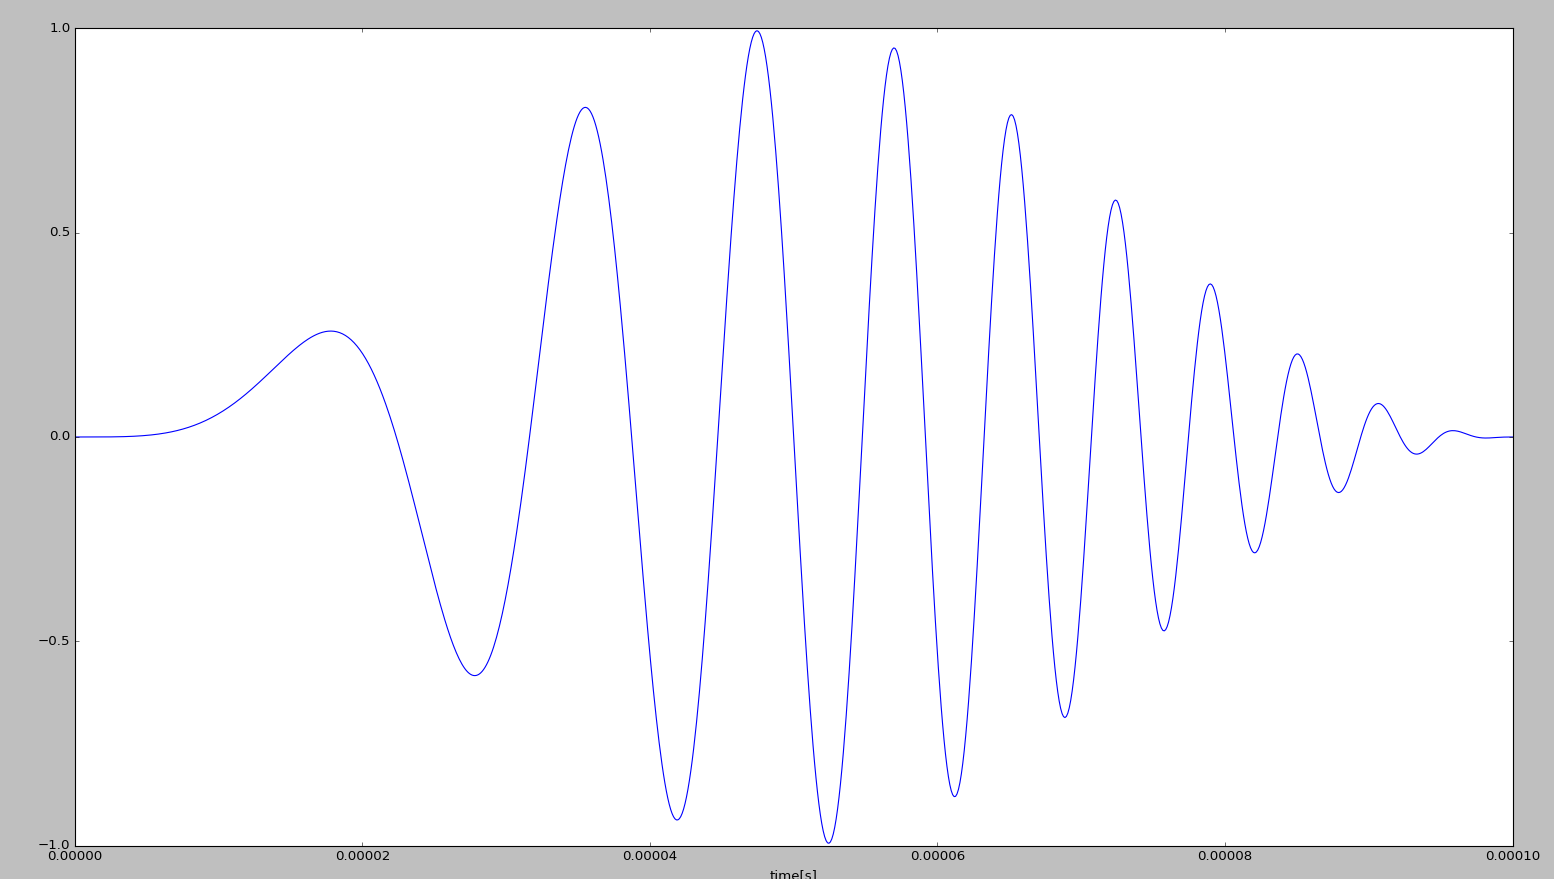
\includegraphics[width=14cm]{Zdjecia/4/test_chirp}
\caption{Algorytm kompensacji odwracania czasu}
\label{fig:sygnal we}
\end{figure}
Wygenerowany przez aplikację sygnał jest różny dla różnych zadanych odległości. Obrazuje to rysunek \ref{fig:rozne_odl} na którym przedstawiono sygnały mające się skompensować odpowiednio po 1, 2, 3, 4 metrach, gdy propagują pierwsze cztery postaci fali prowadzonej. 
\begin{figure}[h]
\centering
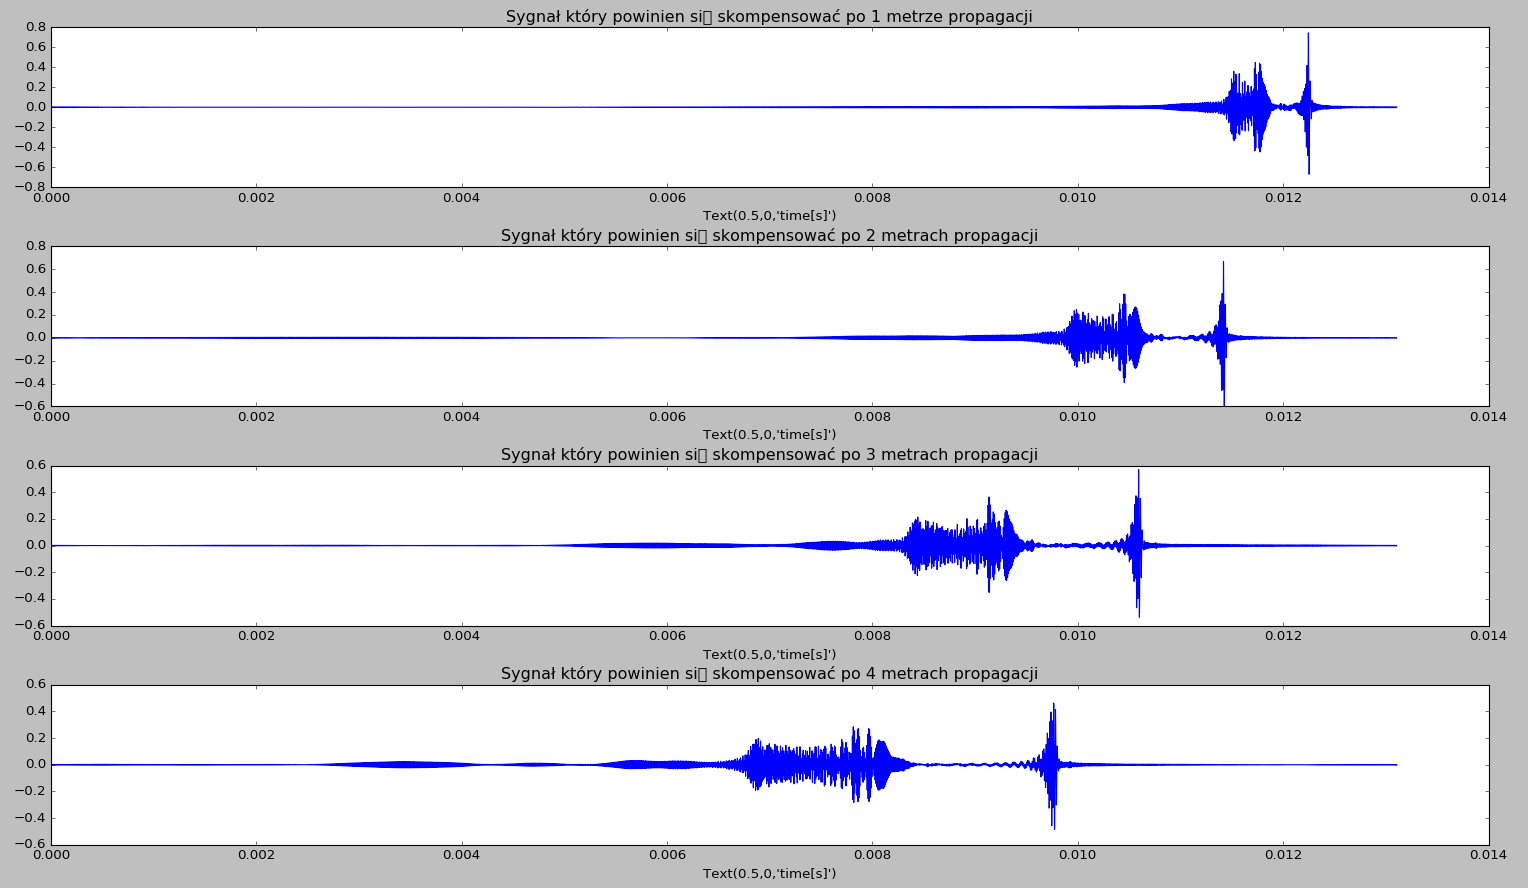
\includegraphics[width=14cm]{Zdjecia/4/tr_przykl}
\caption{Sygnał przygotowany do kompensacji po odpowiedno 1,2,3 oraz 4 metrach}
\label{fig:rozne_odl}
\end{figure}
Sygnał jest też różny dla różnej ilości propagujących trybów, rysunek \ref{fig:rozne_tryby}. Jak łatwo zauważyć, im większa ilość propagujących postaci tym bardziej widoczne staje się zjawisko dyspersji i tym dłuższy staje się przepropagowany sygnał.
\begin{figure}[h]
\centering
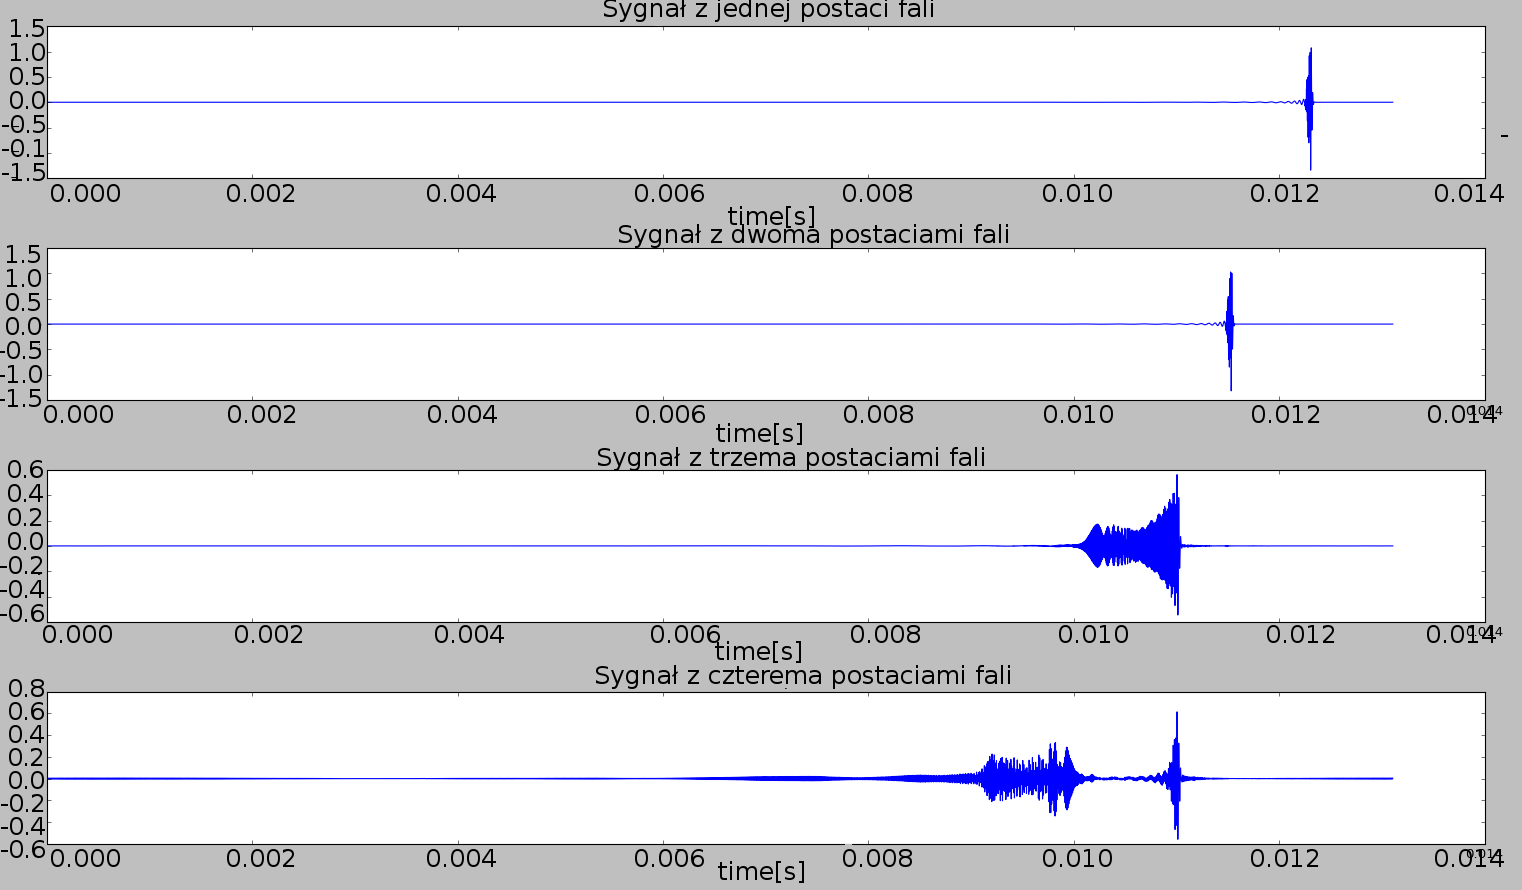
\includegraphics[width=14cm]{Zdjecia/4/TR-rozna_ilosc_modow}
\caption{Sygnał przygotowany do kompensacji po 2,5 metra propagacji zawierający kolejno 1,2,3 oraz 4 postaci fali prowadzonej}
\label{fig:rozne_tryby}
\end{figure}
Tak wygenerowane sygnały zostały przetestowane przez propagację w symulacji. Rysunek \ref{fig:100} ilustruje jak ważna jest znajomość długości ścieżki propagacji. Jeśli sygnał przebędzie zbyt krótką lub zbyt długą drogę to odebrany sygnał nie będzie skompensowany.
\begin{figure}[h]
\centering
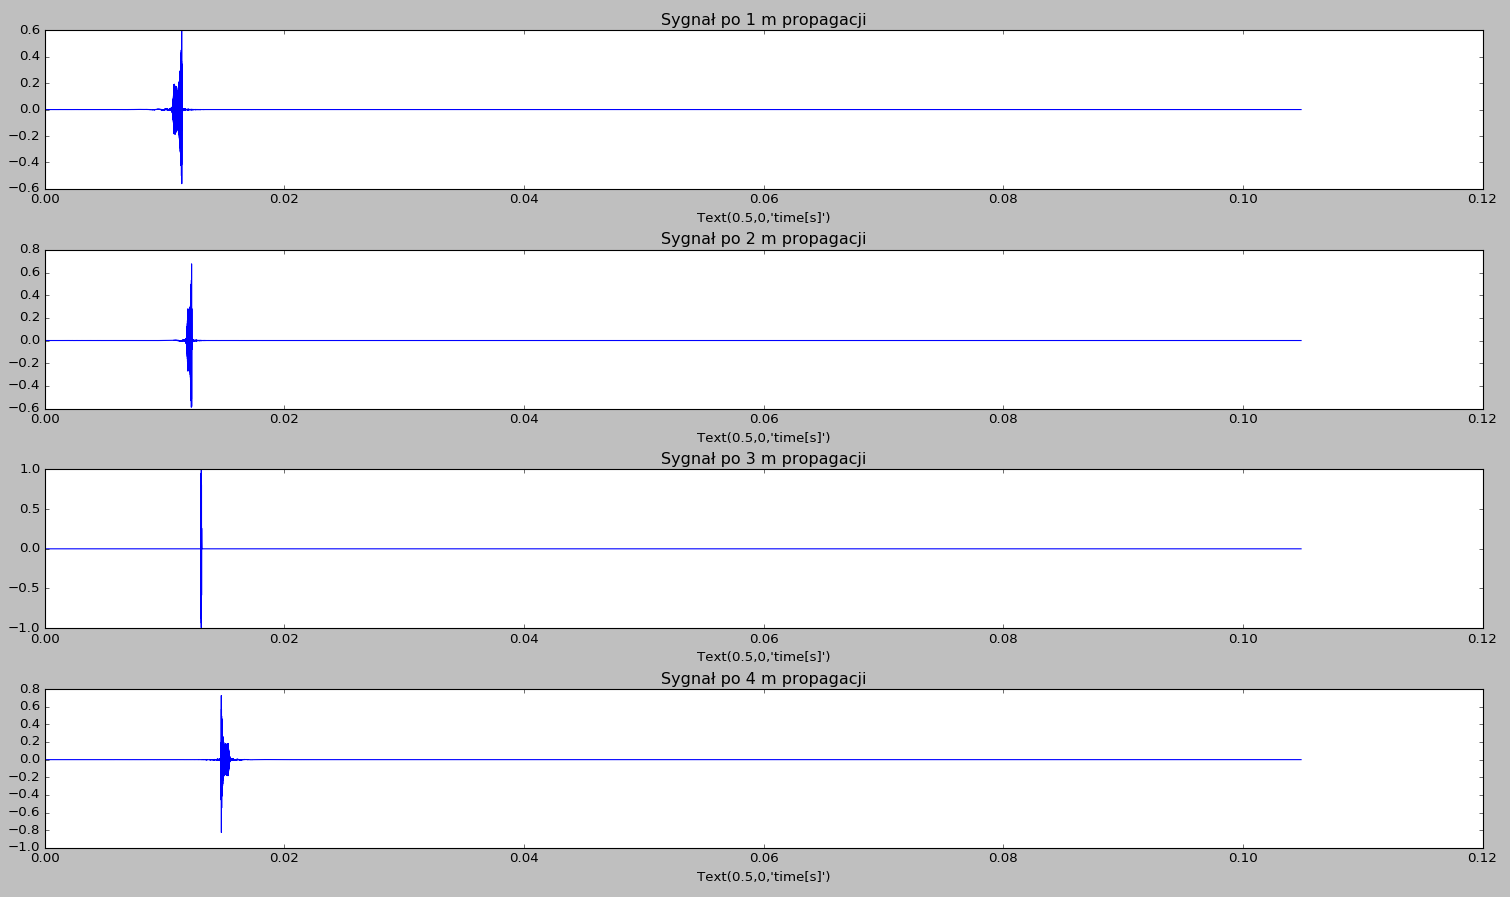
\includegraphics[width=14cm]{Zdjecia/4/obrazek100}
\caption{Sygnał przygotowany do kompensacji po 3 metrach propagacji przepropagowany kolejno o 1,2,3 i 5 metrów}
\label{fig:100}
\end{figure}
Rysunek \ref{fig:skompensowane_TR} ilustruje wyniki symulacji propagacji na odpowiednie odległości sygnałów przedstawinych na rysunku 4.9
\begin{figure}[h]
\centering
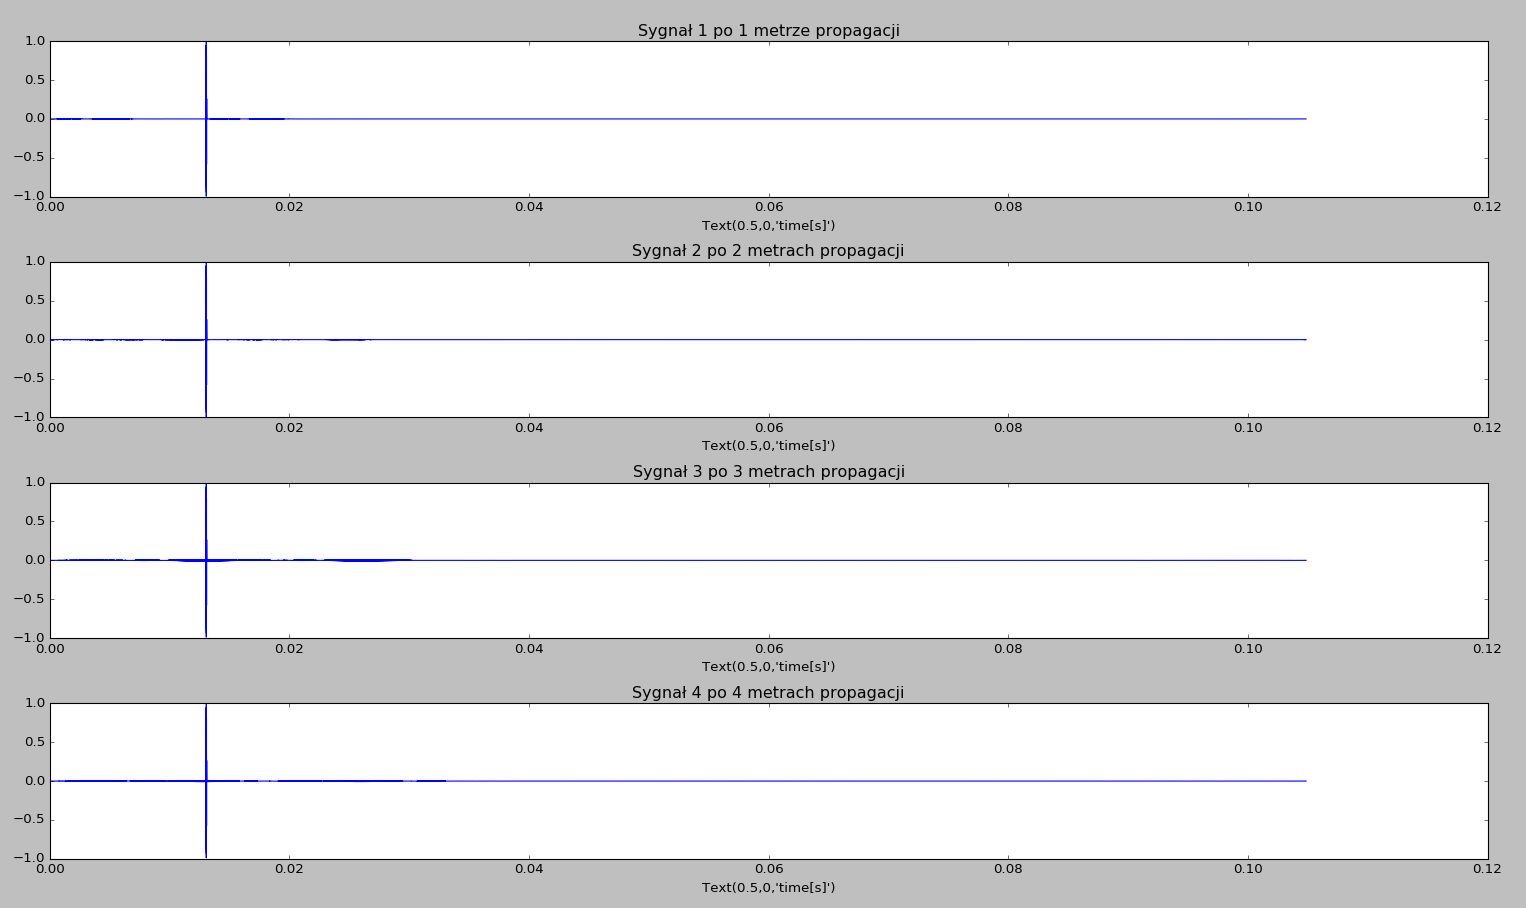
\includegraphics[width=14cm]{Zdjecia/4/skompensowane_TR}
\caption{Sygnały  z rysunu 4.9 po przepropagowaniu odpowiednich odległości}
\label{fig:skompensowane_TR}
\end{figure}

Rysunek \ref{fig:tr_rozna_il_postaci_skomp} ilustruje wyniki  symulacji propagacji sygnałów przedstawionych na rysunku 4.10. Łatwo zauważyć, że wyniki symulacji dają bardzo dobre rezultaty. 
\begin{figure}[h]
\centering
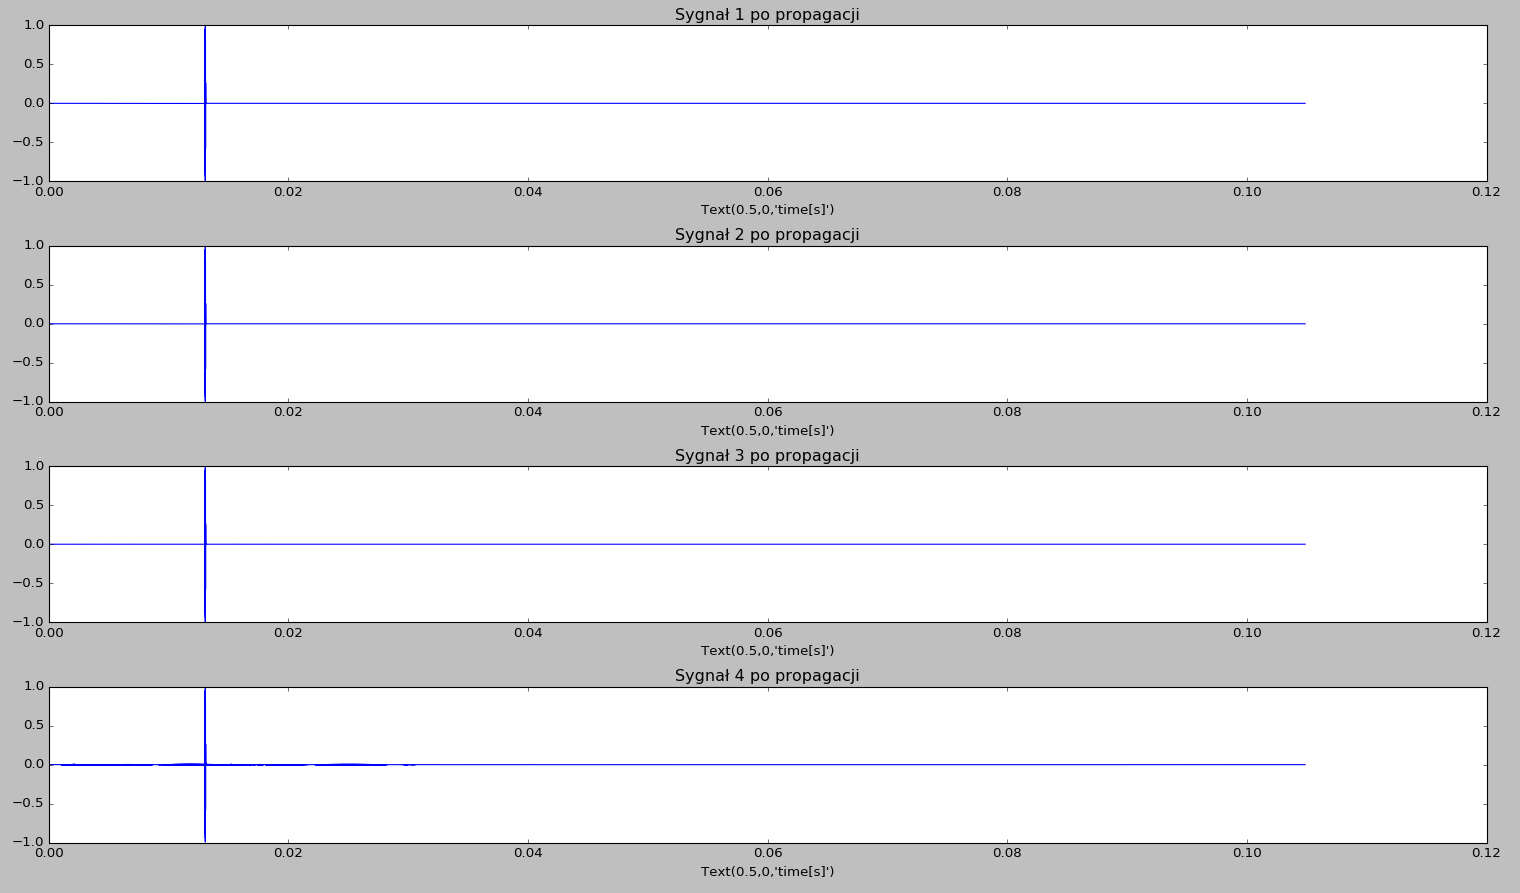
\includegraphics[width=14cm]{Zdjecia/4/tr_rozna_il_postaci_skomp}
\caption{Sygnały  z rysunu 4.10 po przepropagowaniu odpowiedniej odległości}
\label{fig:tr_rozna_il_postaci_skomp}
\end{figure} 

Rysunek \ref{fig:porownanie} przedstawia porównanie wyniku symulacji sygnału linear chirp po propagacji dwóch metrów w pręcie w którym propagowały trzy pierwsze tryby fali prowadzonej (kolor niebieski) oraz sygnału wygenerowanego w aplikacji, przygotowanego do kompensacji po dwóch metrach. Łatwo zauważyć, że przedstawiana metoda pozwala znacząco skrócić czas trwania odbieranego sygnału. Sygnał bez kompensacji trwa 6e-4s natomiast z 1e-4 czyli dokładnie tyle ile żądany sygnał. A zatem można stwierdzić iż kompensacja została skutecznie przeprowadzona. Kolejny rysunek przedstawia porównanie sygnału założonego na wejściu, jako jako postać do której powinien on zostać skompensowany, oraz sygnału faktycznie otrzymanego po symulacji propagacji. Czas trwania oraz obwiednia sygnału zgadzają się z założeniami, jednak widać iż otrzymany sygnał jest sygnałem odwróconym w czasie w stosunku do założonego sygnału. Wynik nie jest zatem idealnym odwzorowaniem założeń, niemniej jednak otrzymany sygnał został maksymalnie skompensowany. W otrzymanym sygnale nie ma również widocznych szumów, pogarszających czytelność otrzymanego wyniku. Oczywistym jest fakt, iż w przypadku rzeczywistym szumy z pewnością by występowały. Idealne matematyczne odwzorowanie padanego obiektu nie jest możliwe, lecz mimo to metoda powinna dawać dobre rezultaty.

\begin{figure}[h]
\centering
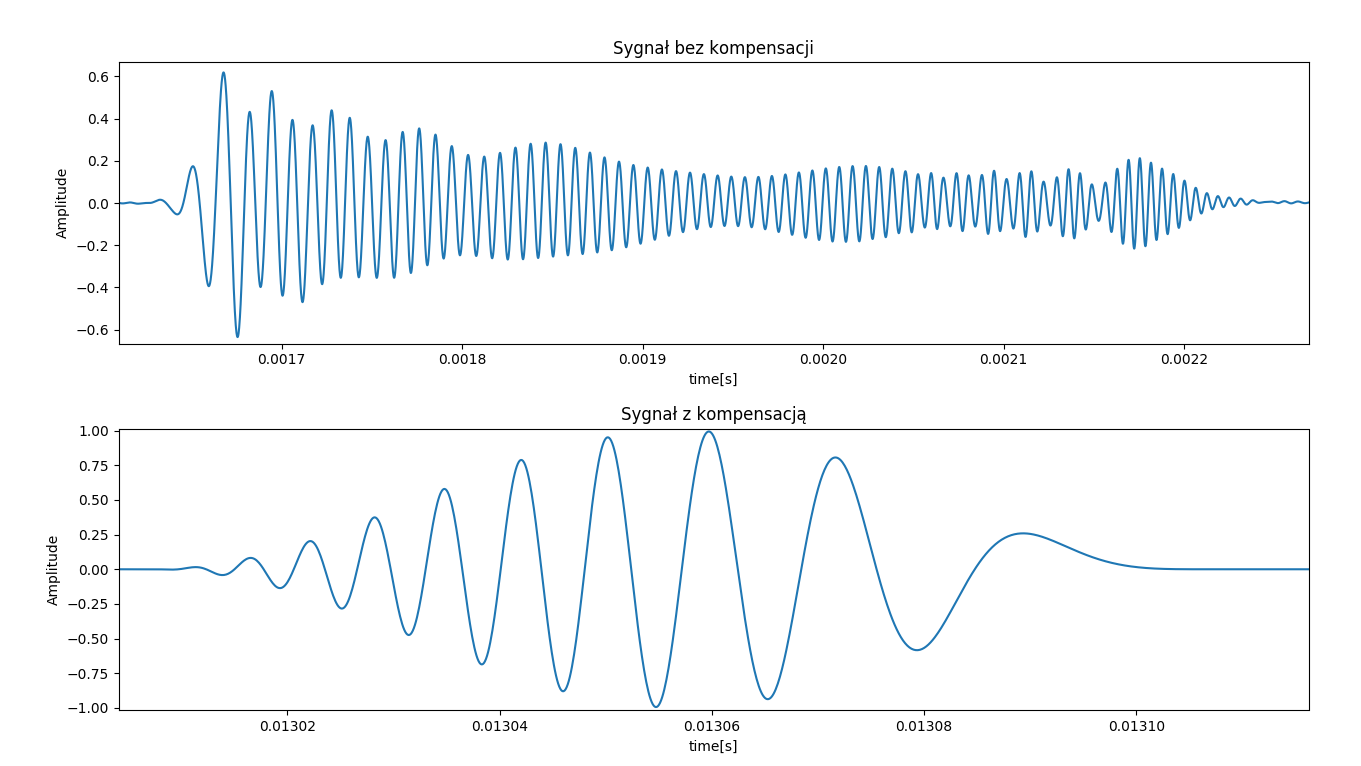
\includegraphics[width=14cm]{Zdjecia/4/tr_porownanie}
\caption{Porównanie sygnału bez kompensacji(górny) oraz z kompensacją (dolny)}
\label{fig:porownanie}
\end{figure} 

\begin{figure}[h]
\centering
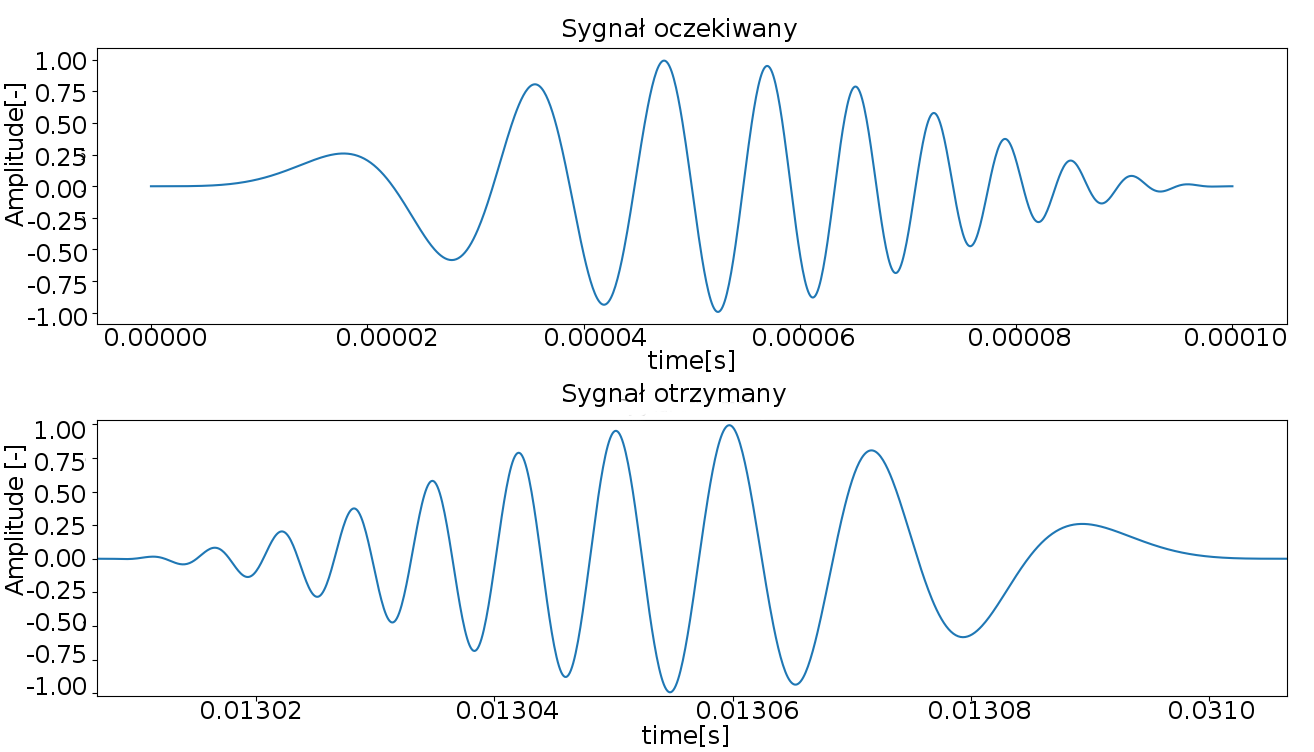
\includegraphics[width=14cm]{Zdjecia/4/tr_porownanie2}
\caption{Porównanie sygnału oczekiwanego(górny) otrzymanego (dolny)}
\label{fig:porownanie2}
\end{figure} 


\section{Metoda mapowania liniowego przy pomocy rozwinięcia w szereg Taylora}
\label{sec:Taylor}
Prezentowana w poniższej sekcji metoda kompensacji dyspersji została przedstawiona w artykule []\textcolor{red}{referenacja do yuanliu}
\subsection{Podstawy teoretyczne}
Po wzbudzeniu badanego pręta odpowiednim sygnałem wejściowym, możliwe jest aby przełączył się on w tryb obioru sygnału i nasłuchiwał nadejścia odpowiedzi układu. W takim wypadku odpowiedź jaką uzyskamy będzie sumą odpowiedzi ze wszystkich odbić, od końca pręta oraz ewentualnych łączeń lub uszkodzeń.  Proponowana w tym rozdziale metoda opiera sie na założeniu, że w badanym obiekce propaguje jedna wybrana postać drgań. Jej celem jest kompensacja powstałej dyspersji, tak aby sygnały z różnych punktów odbicia nie nachodziły na siebie i była możliwa ich interpretacja w celu ustalenia ilości punktów odbicia oraz oszacowania ich odegłości od miejsca wzbudzenia na podstawie znajomości prędkości grupowej fali. Przy tak sformułowanych założeniach, sygnał otrzymany w odbiorniku można przedstawić wzorem:
\begin{equation}
g(t) = \sum\limits_{n=1}{N}f_n(r_n,t)=\frac{1}{2\pi}\int _{-\infty}^{\infty}F(\omega)\sum\limits_{n=1}^{N}(A_n(\omega)e^{-ikr_n})e^{i\omega t} d\omega \label{eq:g(t)_taylor}
\end{equation}
Gdzie:

$N$ - całkowita liczba ścieżek propagacji sygnału (liczba punktów odbicia)

$r_n$ - długość n-tej ścieżki propagacji

$A_n$ - współczynnik odbicia n-tego punktu odbicia.

Widmo częstotliwości takiego sygnału $G(\omega)$  możemy obliczyć przy pomocy transformaty Fouriera i zapisać wzorem:
\begin{equation}
G(\omega) = F(\omega)\sum\limits_{n=1}^{N}(A_n(\omega)e^{-ikr_n} \label{eq:G(omega)_taylor}
\end{equation}

Jak wiadomo, dyspersja zależy od kształtu krzywej dyspersji, $k = K(\omega)$. Jeśli więc $K(\omega)$ jest funkcją kwadratową lub wyższego rzędu względem $\omega$, to $G(\omega)$ reprezentuje widmo częstotliwości rozproszonych pakietów fal. Jeśli natomiast zależność $K(\omega)$ byłoby funkcją liniową, zjawisko dyspersji nie występowałoby, a $G(\omega)$ reprezentowałoby widmo częstotliwości sygnału, który nie uległ dyspersji. 
Wybraną krzywą dyspersji można przybliżyć przy pomocy rozwinięcia w szereg Taylora:
\begin{equation}
k = K(\omega) - k_0+k_1(\omega - \omega _0) + k_2(\omega - \omega _0^2)+... \label{eq:szereg_k}
\end{equation}

Gdzie:

$k_0 = \frac{\omega _0}{c_p}$

$k_1 = \frac{dk}{d\omega}|_{\omega = \omega_0}$

$k_2 = \frac{1}{2}\frac{d^2k}{d\omega ^2}|_{\omega = \omega _0}$

$c_p$ - prędkość fazowa

Wynika z tego, iż dyspersję sygnału można usunąć usuwając jej nieliniowy składnik, poprzez zastąpienie oryginalnej zależności $K(\omega)$ liniowym przybliżeniem tej funkcji. Zastosowanie takiego zabiegu sprawi, iż sygnał w dziedzinie czasu będzie postrzegany jako skompensowany do postaci niedyspersyjnej, a prędkość grupowa obliczona z liniowego przybliżenia krzywej dyspersji może zostać wykorzystana do określenia długości ścieżek propagacji wynikających z kolejnych odbić. 

W szczególnym przypadku, w którym mamy do czynienia z pojedyńczą ścieżką propagacji ($N=1$) i odległość między nadajnikiem a punktem odbicia jest znana, można usunąć dyspersję poprzez wyeliminowanie wyrażenia kwadratowego w $K(\omega)$. Matematycznie można to zrobić przy pomocy wzoru:
\begin{equation}
 \widetilde{G}(\omega)=(F(\omega)A_1(\omega)e^{-ikr_1})e^{ik_2(\omega -\omega _0)^2r_1}
\end{equation}

Gdzie $\widetilde{G}(\omega)$ jest zmodyfikowanym widmem częstotliwości, a $r_1$ jest odległością między nadajnikiem i odbiornikiem. Sygnał skompensowany w dziedzinie czasu można natychmiast uzyskać poprzez odwrotną transformatę Fouriera. Ponieważ jednak zazwyczaj długość ścieżki propagacji sygnału nie jest znana, a sygnał może składać się z wielu odbić, między innymi od uszkodzeń ($N>1$) usuwanie dyspersji przy pomocy powyższego wzoru byłoby niepraktyczne. 

Rysunek \ref{fig:krzywa_taylorem} obrazuje przykład krzywej dyspersji, trybu $A_0$, płyty aluminiowej o grubości 3,175 mm. Linia ciągła pokazuje zależności $K(\omega)$ uzyskaną metodami komputerowymi, natomiast linia przerywana kropkowana wskazuje z rozwinięcie szeregu Taylora pierwszego rzędu, a linia przerywana rozszerzenie szeregu Taylora drugiego rzędu w odniesieniu do centralnej częsości kątowej ($\omega _0 = 2\pi *50 kHz$)

\begin{figure}[h]
\centering
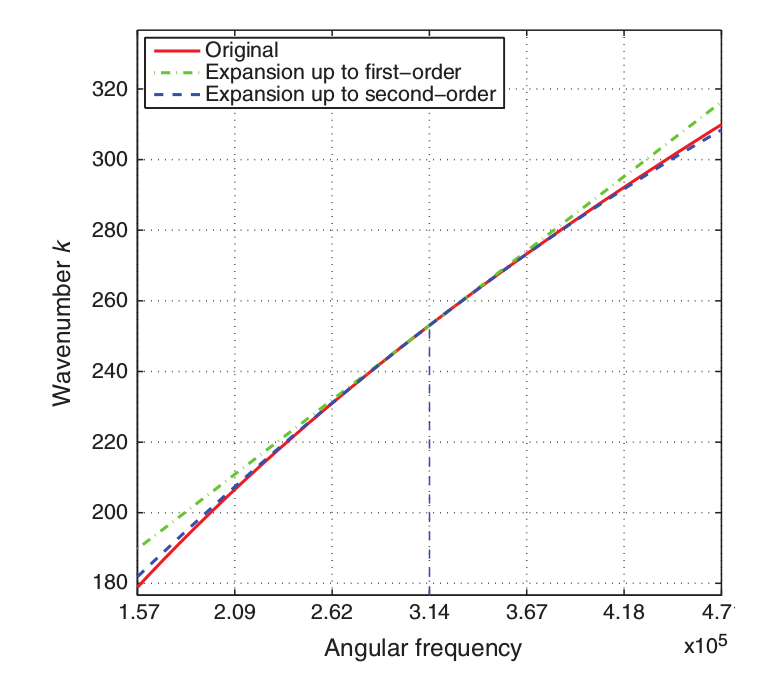
\includegraphics[width=14cm]{Zdjecia/4/buba}
\caption{Przykładowe porównanie oryginalnej krzywej oraz jej przybliżeń przy pomocy rozwinięcia w szereg Taylora}
\label{fig:krzywa_taylorem}
\end{figure}

Łatwo zauważyć, że po pierwsze, rozszerzenie drugiego rzędu daje bardzo dobrze przybliżenie pierwotnego kształtu krzywej, po drugie, $K(\omega)$ jest monotoniczną funkcją $\omega$ w otoczeniu $\omega _0$. 

Równanie \ref{eq:G(omega)_taylor} można zapisać w postacji złożenia funkcji:
\begin{equation}
G(\omega) = G(k)\circ K(\omega)
\end{equation}

Gdzie $\circ$ jest operatorem składania funkcji. $G(k)$ jest niejawną funkcją k z równania \ref{eq:G(omega)_taylor}. Zamieniając $K(\omega)$ na $K_{lin}(\omega)$ będące aproksymacją $K(\omega)$ pierwszego rzędu w punkcie $\omega _0$, gdzie $\omega _0$ oznacza częstotliwość o najwyższej energii, można wyprowadzić zmodyfikowane widmo częstotliwości:
\begin{equation}
\widetilde{G}(\omega) = G(k)\circ K_{lin}(\omega)
\end{equation}

Ponieważ $G(\omega)$ jest znane oraz znana jest analizowana krzywa dyspersji, znane jest również $G(k)$, obliczając przybliżenie liniowe $K_{lin}(\omega)$ można w prosty psosób obliczyć $\widetilde{G}(\omega)$, poprzez interpolację odpowiednich wartości. Opisana metoda może być określana mianem mapowania liniowego. W jej efekcie uzyskane zostaje nowe widmo częstotliwości $\widetilde{G}(\omega)$. Po mapowaniu widmo amplitudy pozostaje bez zmian, natomiast widmo fazy stopniowo odbiega od pierwotnego w miarę oddalania się od wybranej, środkowej częstotliwości, co dobrze ilustruje rysynek \ref{fig:widma}

\begin{figure}[h]
\centering
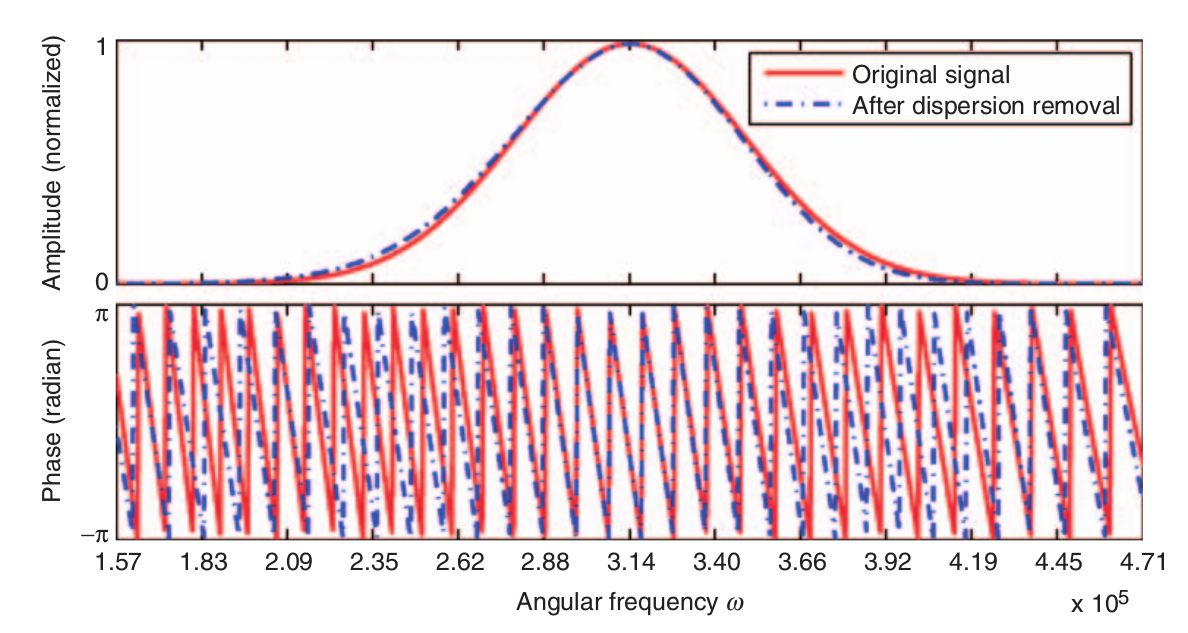
\includegraphics[width=14cm]{Zdjecia/4/widma}
\caption{Przykładowe porównanie oryginalnych charakterystyk oraz ich przybliżeń przy pomocy rozwinięcia w szereg Taylora}
\label{fig:widma}
\end{figure}

Należy zaznaczyć, iż stosowanie omawianej metody jest możliwe tylko w sytuacji, gdy $K(\omega)$ jest funkcją monotoniczną

\subsection{Implementacja numeryczna}
Implementacja prezentowanej metody opiera się głównie na znajomości krzywej dyspersji, której propagację bierzemy pod uwagę. Pierwszym krokiem, jest wygenerowanie odpowiedniego sygnału testowego. Mając właściwy sygnał można przystąpić do właściwego procesu kompensacji. W pierwszej kolejności analizowane jest widmo amplitudowe otrzymanego sygnału. Na jego podstawie uzyskiwana jest informacja o częstotliwości z największą energią. Zostaje ona wybrana na częstotliwość w której nastąpi przybliżenie liniowe. Po wybraniu $\omega _0$ odnajdywane jest na krzywej dyspersji odpowiednia wartość liczby falowej. Korzystając z zależności opisujących wartości $k_0$ i $k_1$ wyliczone zostaje liniowe przybliżenie badanej krzywej. Uzyskane w aplikacji wyniki przedstawia rysunek \ref{fig:krzywa_moja}. Linia niebieska prezentuje oryginalną krzywą dyspersji, natomiast linia zielona przdstawia jej przybliżenie uzyskane w aplikacji przy użyciu rozwinięcia w szereg Taylora.

\begin{figure}[h]
\centering
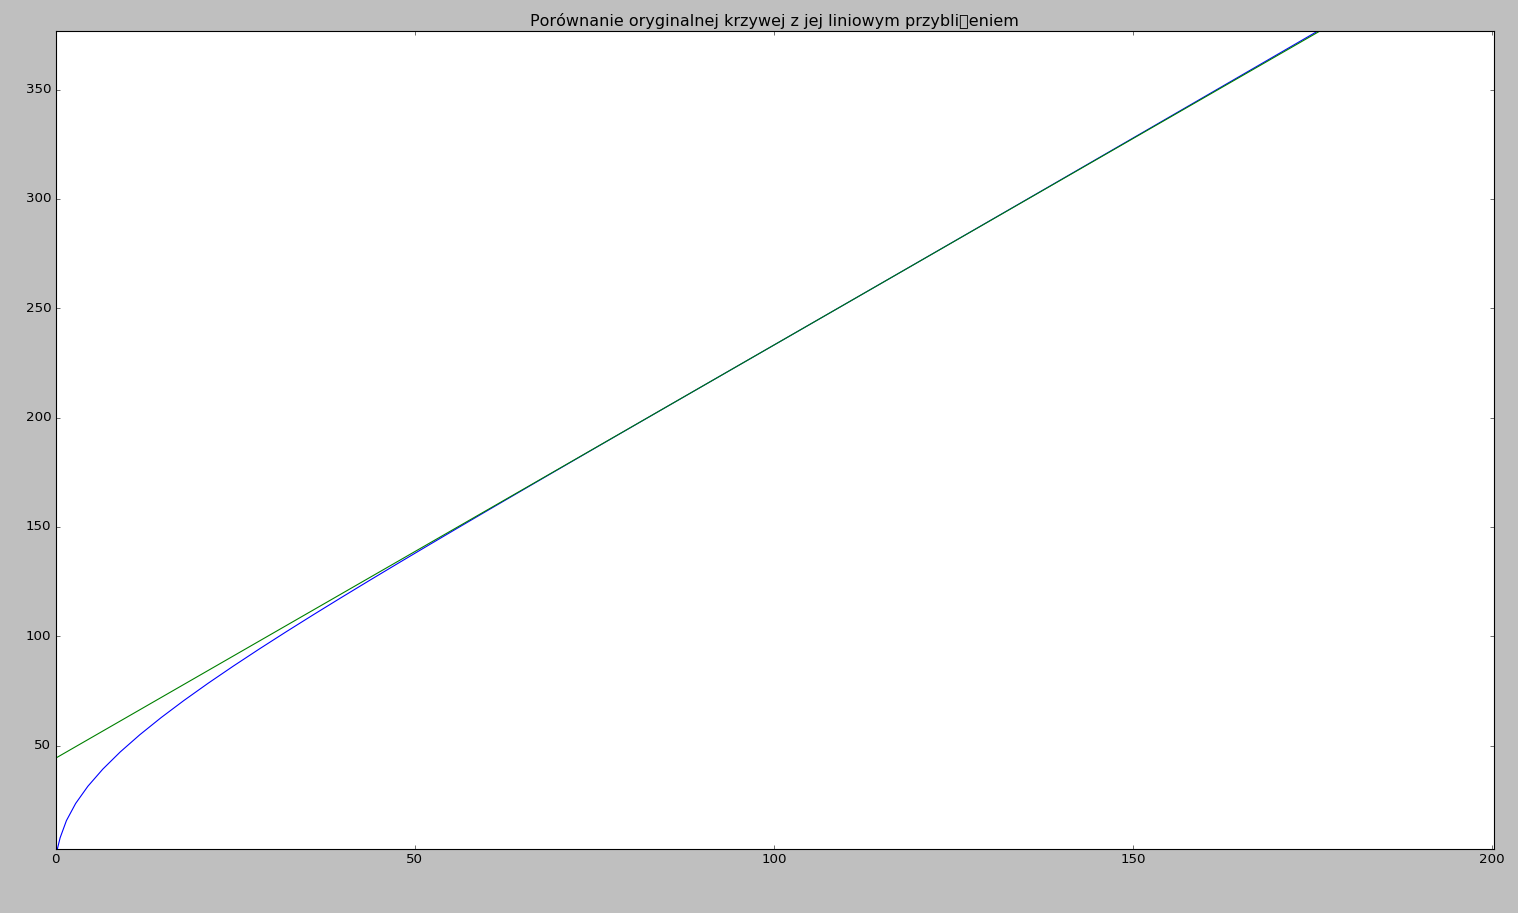
\includegraphics[width=14cm]{Zdjecia/4/krzywa_moja}
\caption{Przykładowe porównanie oryginalnej krzywej oraz jej przybliżeń przy pomocy rozwinięcia w szereg Taylora}
\label{fig:krzywa_moja}
\end{figure}

Kolejnym krokiem implementowanego algorytmu, jest wyliczenie G(k) na podstawie otrzymanego widma sygnału $G(\omega)$ na podstawie krzywej dyspersji. Następnie ponowne wyznaczenie zależności w dziedzinie częstotliwości, tym razem jednak używając przybliżenia liniowego zamiast oryginalnej krzywej dyspersji. Omawiany algorytm doskonale ilustruje rysunek \ref{fig:algo_Taylora}

\begin{figure}[h]
\centering
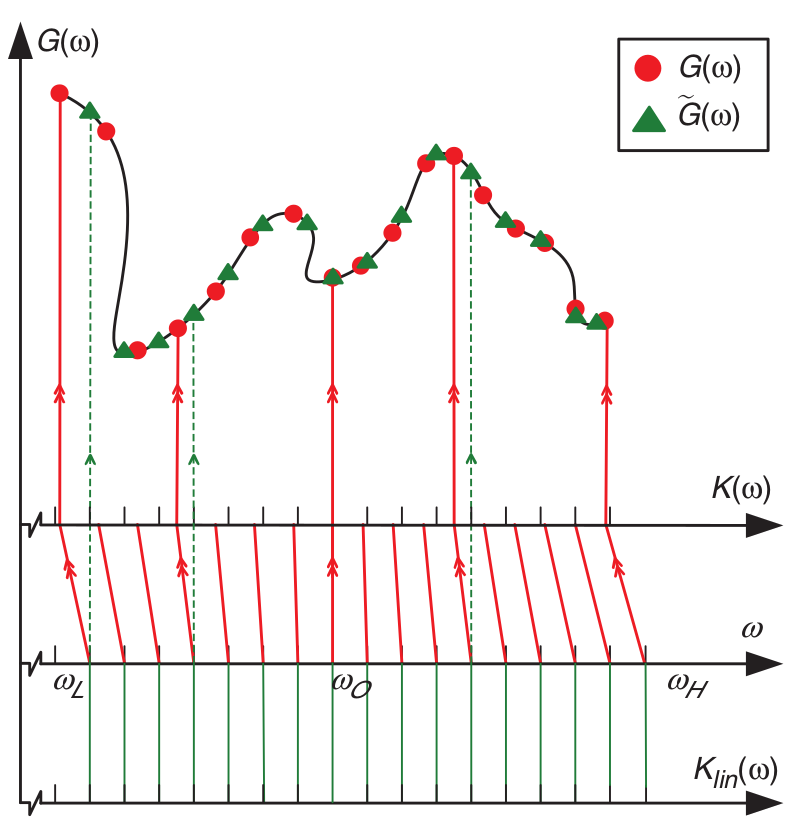
\includegraphics[width=13cm]{Zdjecia/4/algo_Taylora}
\caption{Wizualizacja algorytmu []Przypis do Pialucha}
\label{fig:algo_Taylora}
\end{figure}

Przedstawia on krzywą $G(\omega)$ z aż trzema osiami poziomymi. Linia ciągła przedstawia zależność $G(K(\omega))$, czerwonymi kółkami oznaczony jest sygnał $G(\omega)$. Jak widać przejście z dziedziny $K(\omega)$ na $\omega$ jest nieliniowe co wynika z niliniowego charakteru krzywej dyspersji. Zielonymi trójkątami oznaczono natomiast krzywą $G(K_{lin}(\omega))$. Jak widać przejście z dziedziny $\omega$ na $K_{lin}(\omega)$ jest przejściem o charakterze liniowym. 
\subsection{Wybrane wyniki symulacji}
Rysunek \ref{fig:liniakrzyws} obrazuje przybliżenie krzywej dyspersji wyznaczonej dla zadanego sygnału z rysunku 4.8.
\begin{figure}[h]
\centering
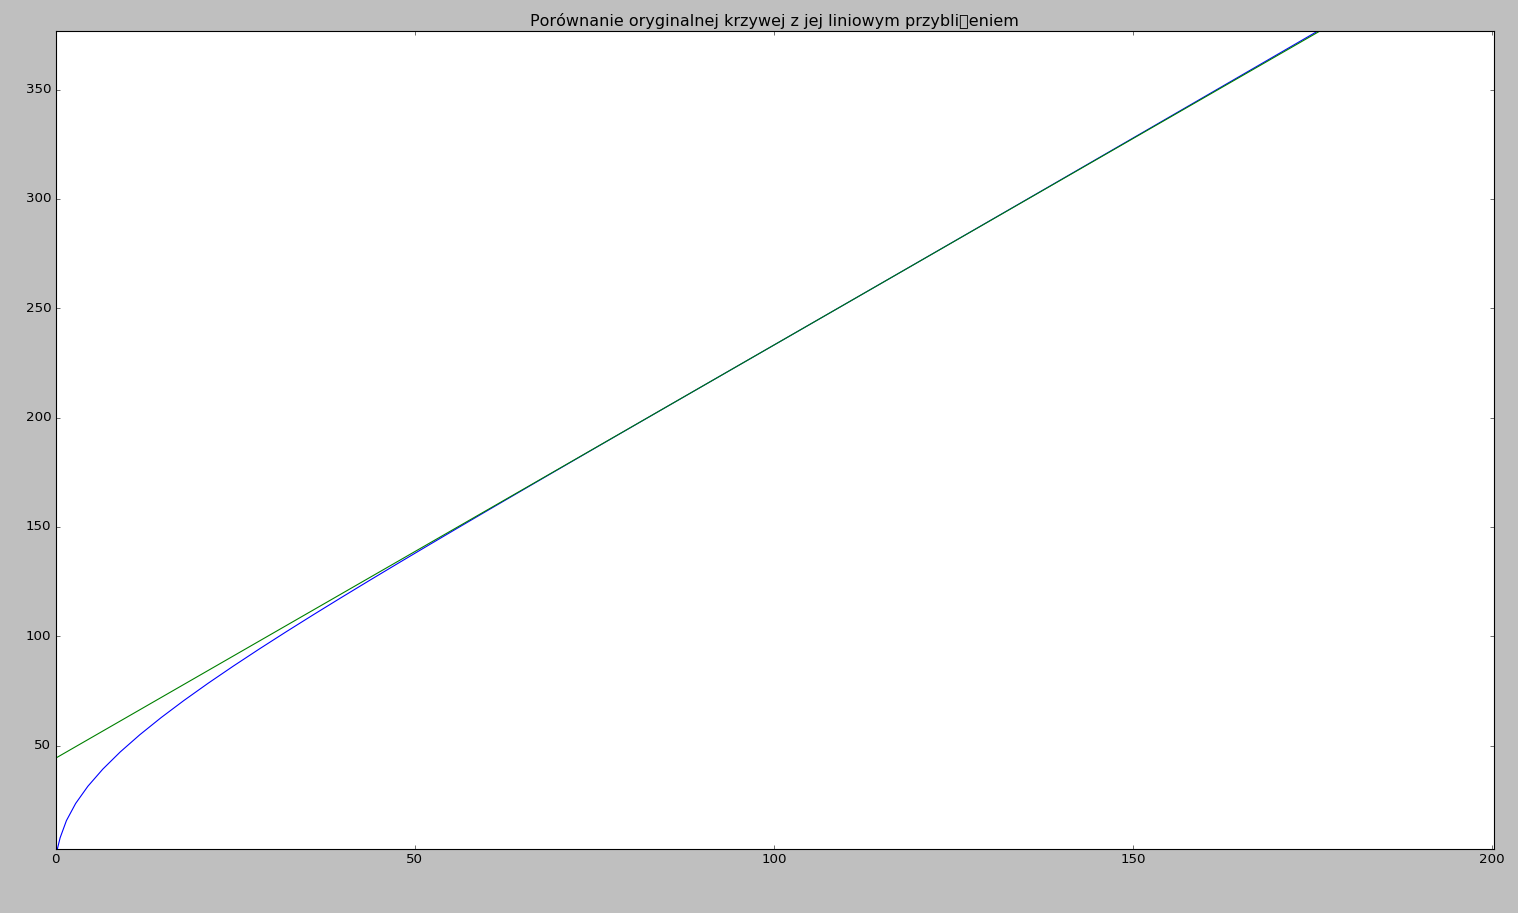
\includegraphics[width=13cm]{Zdjecia/4/krzywa_moja}
\caption{Porównanie oryginalnej krzwej z jej liniowym przybliżeniem}
\label{fig:liniakrzyws}
\end{figure}
Rysunek \ref{fig:przedipo} ilustruje przykład sygnału przed i po kompensacji.
\begin{figure}[h]
\centering
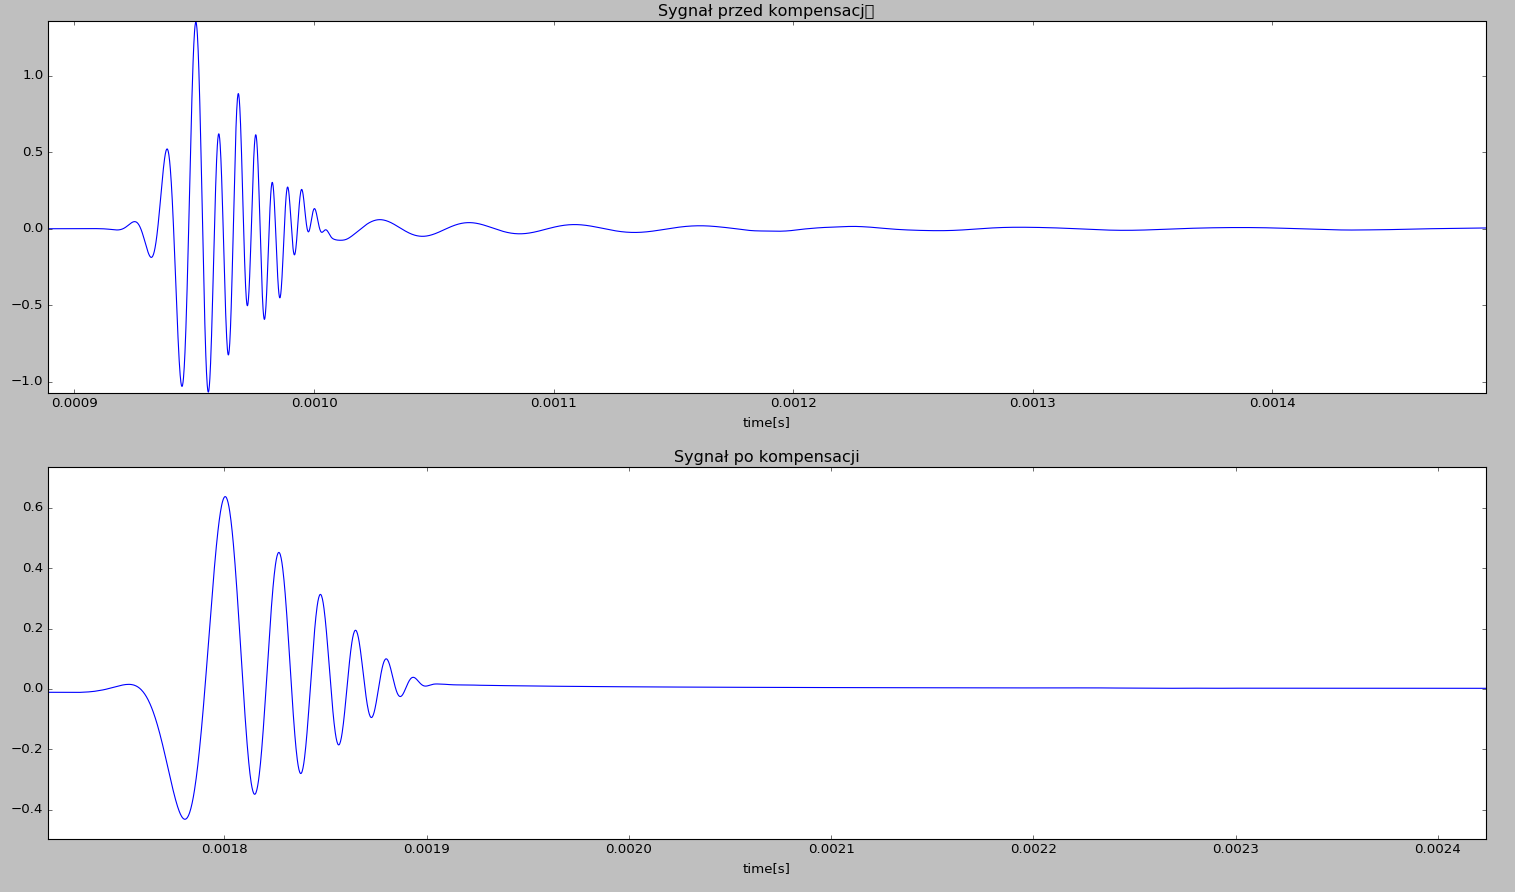
\includegraphics[width=13cm]{Zdjecia/4/przedipo}
\caption{Porównanie sygału przed i po kompensacji}
\label{fig:przedipo}
\end{figure}
Na ostatnim rysunku przedstawione zostało porównanie otrzymanych w wyniku kompensacji sygnałów z sygnałem zadanym \ref{fig:przedipo2}
\begin{figure}[h]
\centering
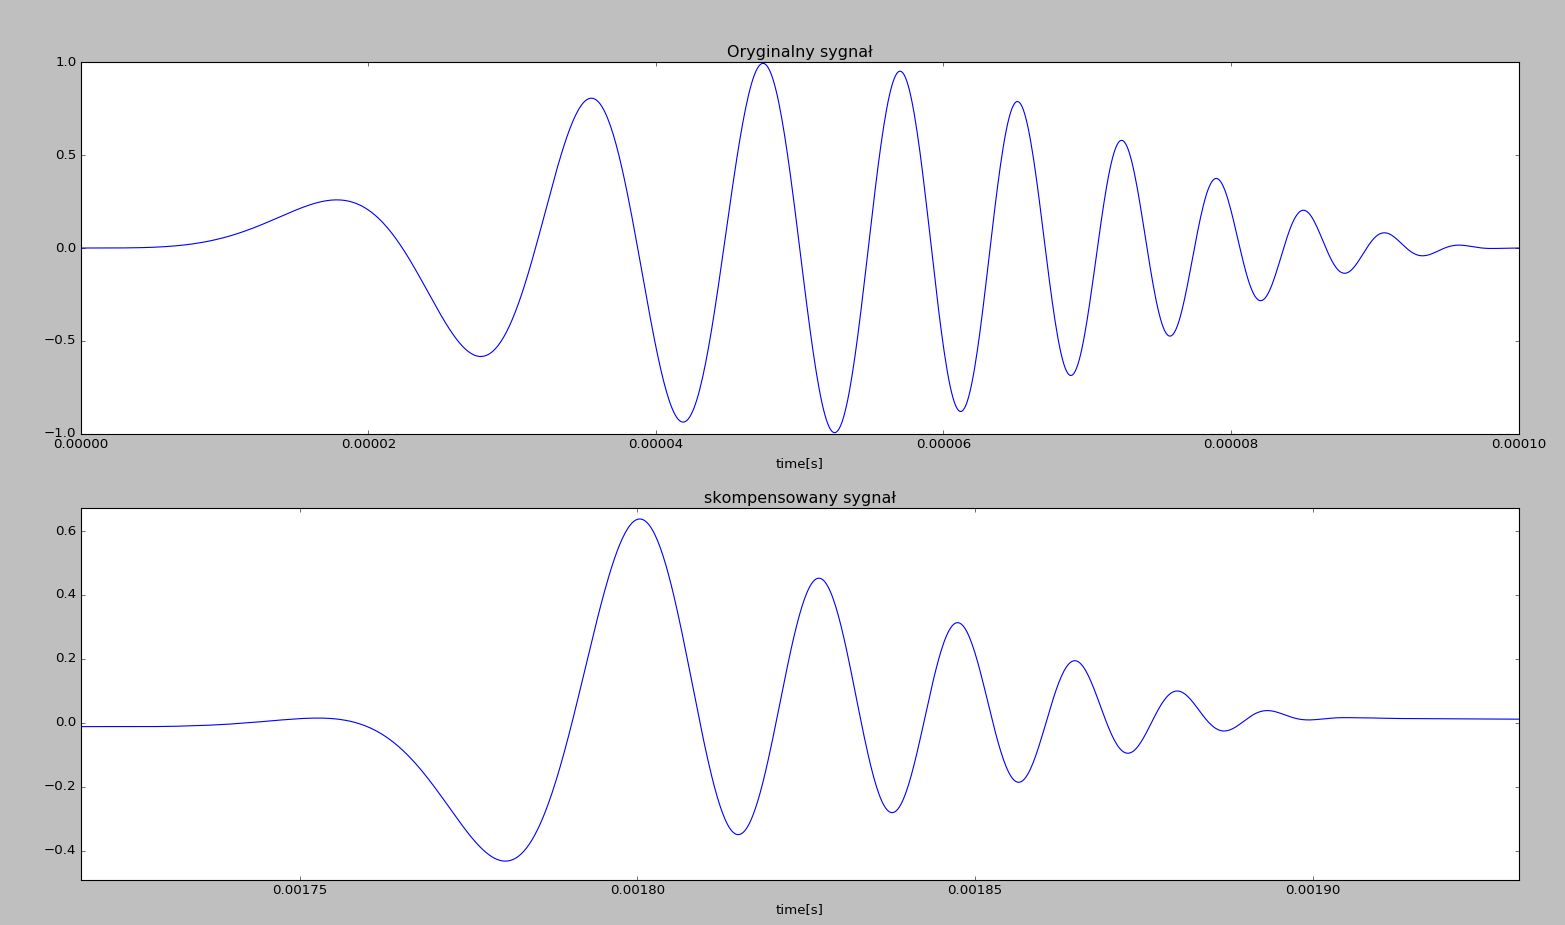
\includegraphics[width=13cm]{Zdjecia/4/przedipo2}
\caption{Porównanie sygnału oryginalnego z sygnałem skompensowanym}
\label{fig:przedipo2}
\end{figure}

%\input{4_x_Metoda_taylora}
%\input{4_5_Metoda_mapowania_sygnału_z_dziedziny_czasu_na_dziedzinę_odległości}
%\input{4_6_Porównanie_opracowanych_metod_kompensacji}
